\documentclass{article}
\usepackage[a4paper, total={6in, 8in}]{geometry}
\usepackage[utf8]{inputenc}
\usepackage{latexsym}
\usepackage{amsmath}
\usepackage{pgfplots}
\usepackage{amsfonts}
\usepackage{mathtools}
\usepackage[export]{adjustbox}
\usepackage{wrapfig}
\usepackage{chngcntr}
\usepackage{float}
\usepackage{todonotes}
\usepackage{tikz}
\pgfplotsset{compat=1.17}
\usepackage{csquotes}
%\usepackage[dvipsnames]{xcolor}
\usetikzlibrary{ decorations.markings}
\newtheorem{theorem}{Theorem}[section]
\newtheorem{definition}{Definition}[section]
\newtheorem{corollary}{Corollary}[theorem]
\newtheorem{lemma}[theorem]{Lemma}
\newtheorem{proposition}{Proposition}[theorem]
%\newtheorem*{remark}{Remark}

\usepackage[english]{babel}
\usepackage{biblatex}
\addbibresource{mylib.bib}

\numberwithin{equation}{section}
\pagenumbering{gobble}

\title{A brief endeavour into traffic modelling}

\author{Camilla Balestrand Klemetsen}

\date{Spring 2021}

\begin{document}

\maketitle
%\addFrontPage
\newpage
\pagenumbering{roman}
%\begin{abstract}
%    PDEs are very interesting :-)) %and cool
%\end{abstract}

%\newpage

\tableofcontents 

\newpage
\pagenumbering{arabic}

\section{Introduction}
A partial differential equation (PDE) is a type of differential equation which contains unknown functions of several variables, and their partial derivatives. These equations are often used in physics and formulated to solve problems of multiple variables, like the spread of heat or waves in a medium, electrostatics- and dynamics, fluid mechanics and many more. It turns out that many physical phenomena can be described by the same generalised mathematical equation, and thus may be governed by the same dynamics.

The behaviour of traffic can be both complex and non-linear. It depends on the amount of vehicles, the speed limits and the individual drivers. Many attempts have been made to produce a mathematical model for traffic flow. A well known approach is the fluid-dynamic model introduced in the $50$s by Lighthill, Whitham and Richards (LWR), where the idea was that the flow of water also could model the flow of traffic. It was simple, and allowed for many phenomena like queue formation and evolution. Since then, many more contributions has been made, but none have been able to accurately describe and model traffic. We are still on the hunt for a more accurate model which can explain the experimental features which we see in real traffic \cite{KernerHelbing}. Today, we see an increasing number of vehicles in modern cities and traffic networks. The presence of traffic lights, roundabouts and stop signs affects the flow of traffic and may lead to hard congestion and bottlenecks. This greatly affects productivity and pollution and more, and thus solutions to these challenges will have socio-economic impact \cite{GaravelloMauro2006Tfon}. Where to place traffic lights or roundabouts, exits and overpasses is one of the main goals in our understanding of traffic. We aim to maximise traffic flow and minimise congestion, accidents and pollution \cite{GaravelloMauro2006Tfon}. 

Imagine flying over a motorway. Below we can see small cars entering the motorway, driving along and then exiting the motorway. If a queue forms, we have a high density of cars, and a decline in average speed of the cars.  And if there is no queue the density of cars can be very low. We can describe the flow of cars on the motorway mathematically, like the flow of a fluid,  where $\Omega$ is the motorway and the entrances and exits are $\partial \Omega$. 

\begin{wrapfigure}[11]{L}{0.3\textwidth}
    \begin{center}
        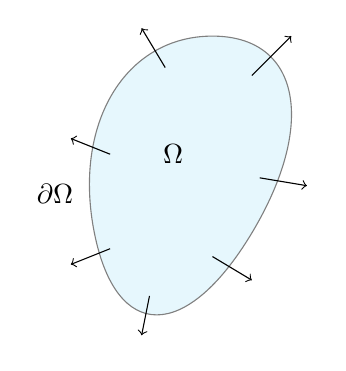
\begin{tikzpicture}
         \filldraw[fill=cyan!10!white, draw=black!50] plot [smooth cycle, tension = 2] coordinates { (0,0) (2,0) (1.5,2.5)};
         \node at (-0.5,0.5) {$\partial \Omega$};
         \node at (1,1) {$\Omega$};
        \draw[->] (2,2) -- (2.5,2.5);
        \draw[->] (0.9,2.1) -- (0.6,2.6);
        \draw[->] (0.2,1) -- (-0.3,1.2);
        \draw[->] (0.2,-0.2) -- (-0.3,-0.4);
        \draw[->] (2.1,0.7) -- (2.7, 0.6);
        \draw[->] (1.5,-0.3) -- (2, -0.6);
        \draw[->] (0.7,-0.8) -- (0.6, -1.3);
       \end{tikzpicture}
    \caption{Domain  $\Omega$}
    \label{Fig:ConservationLaws/Domain}
    \end{center}
\end{wrapfigure}{}
%We will frequently use the following notation. 
%\begin{center}
%\begin{itemize}
%  \item[] $\mathbb{N}$ the set of natural numbers, including 0.
%  \item[]  $\mathbb{Q}$ the set of rational numbers.
%  \item[]  $\mathbb{R}$ the set of real numbers.
%  \item[]  $L_{loc}^p $ the set of locally integrable functions.
%  \item[]  $C^0 $ the set of continuous functions.
%  \item[]  $C^1 $ the set of continuous and differentiable functions.
%\end{itemize}
%\end{center}

Let $\Omega \subseteq \mathbb{R}$ and assume $\Omega$ to be a bounded domain with piecewise $C^1$ boundary $\partial \Omega$. Imagine a fluid or the amount of cars inside $\Omega$ with density $\rho = \rho(\boldsymbol{x}, t)$. The fluid might have a velocity $v = v(\boldsymbol x, t)$, and we can describe the the fluid inside the domain as follows:

\begin{equation}
    \underbrace{\frac{d}{dt} \int_{\Omega} \rho dx }_{ \text{The change of mass over time}}  = \underbrace{\int_{\partial \Omega} (\rho v) \cdot n ds }_{\text{The flow of mass over the boundary}}
\end{equation}

Assuming $\frac{\partial \rho}{\partial t}$ is continuous in time and space, we use Leibniz rule and move the differentiation inside the integral. Furthermore, using the divergence theorem on the right hand side: 

\begin{equation}
    \int_{\Omega} \frac{\partial \rho}{\partial t} dx   = - \int_{\Omega} \nabla \cdot (\rho v)dx 
\end{equation}

\begin{equation}
    \int_{\Omega} \big ( \frac{\partial \rho}{\partial t}  + \nabla \cdot (\rho v) \big ) dx   = 0 
\end{equation}

And since the domain is arbitrary: 

\begin{equation}
    \frac{\partial \rho}{\partial t}  + \nabla \cdot (\rho v) = 0
\label{Burgers}
\end{equation}

One should also notice that \textit{only} two simple assumptions were made, conservation of mass, and sufficient smoothness. 

We will use the more general formulation, $u \in \mathbb{R}^n, f \in \mathbb{R}^m$ 

\begin{equation}
    u_t + f(u)_x = 0 
    \label{Equation}
\end{equation}

Where the flux function $f(u)$ will give rise to different models. The one derived above is named the Lighthill-Whitham-Richards (LWR) model. We also have systems of equations, which give rise to models like the Payne-Whitham Model, the Aw-Rascle Model, and multi population models a long with third lane and multi-lane models. 

But before diving into our choice of model, we will start with some theory of non-linear hyperbolic conservation laws.

% ----------------------------------------
% ----------------------------------------
% ----------------------------------------

\section{Non-Linear Hyperbolic Conservation laws}
When given a non-linear conservation law of the form \ref{Equation}, our first instinct is to solve it the \textit{classical} way, by method of characteristics. However, in many cases we cannot expect to find classical solutions for all times using this method, as often the solution evolves into a multi-valued function of $x$.
%Looking at the specific case of the scalar equation \ref{Burgers}, when using the method of characteristics with initial data given by $\rho_0(x) = \rho(x,0) = - arctan(x),  t_0 = 0$, the solution results in a multi valued function of $x$. For that reason, we are not able to define a classical solution for all times $t$. 
Therefore, we will extend our admissable set of solutions in order to allow such discontinuities; so-called weak solutions \cite{HoldenH.Helge2015Ftfh}. 

Consider the model equation \ref{Equation} and let $\phi \in C_0^{\infty}(\Omega \times [0, T])$ have compact support, and assume initial condition $u|_{t=0} = u_0 $. Integrating over an arbitrary domain $[0,T] \times \Omega \subseteq \mathbb{R}$, multiplying with the test function $\phi$, and integrating by parts we get

\begin{align}
    0 &= \int_0^T \int_{\Omega} (u_t + f(u)_x)\phi dxdt \\
      &= \int_0^T \int_{\Omega} (u \phi_t + f(u)\phi_x) dxdt + \int_{\Omega} u_0 \phi(x,0) dx 
    \label{Weak form}
\end{align}

Note that, as $\phi$ has compact support, the boundary terms vanish. Also we no longer have a requirement on $u$ and $f(u)$ to be differentiable. And lastly note that if the equation \ref{Equation} admits a classical solution $u$, then $u$ will also be a solution to the weak formulation \ref{Weak form}. Does this weak solution allow for the discontinuities we require?
\begin{wrapfigure}[12]{L}{0.5\textwidth}
    \begin{center}
        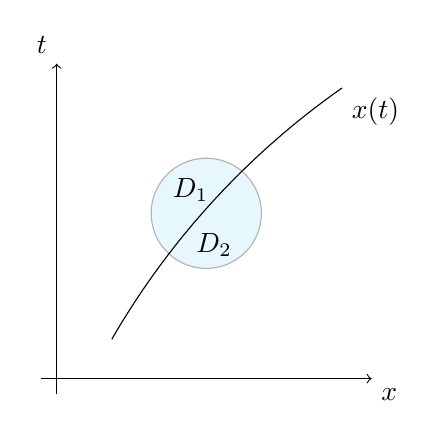
\begin{tikzpicture}
        % coordinate sys
        \draw[->] (0,-0.2) -- (0,4) node[anchor=south east] {$t$};
        \draw[->] (-0.2,0) -- (4,0) node[anchor=north west] {$x$};
        
        % plot
        \filldraw[fill=cyan!10!white, draw=black!30] (1.9, 2.1) circle (0.7cm);
        \node at (1.7,2.4) {$D_1$};
        \node at (2,1.7) {$D_2$};
        \draw (0.7,0.5) arc (150:125:10cm) node[anchor=north west] {$x(t)$};
        \end{tikzpicture}
        \label{fig:ConservationLaws/Isolated_disc}
        \caption{An isolated discontinuity}
    \end{center}

\end{wrapfigure}{}


    
Assume a discontinuity a long a smooth curve $\Gamma : x = x(t)$, which is differentiable in a neighbourhood of $x(t)$, and that the equation $\ref{Equation}$ admits a classical solution outside the discontinuity. Now we choose a neighbourhood $D = D_1 \cup D_2$ around the point $(x(t), t)$, see Figure \ref{fig:ConservationLaws/Isolated_disc}, and a test function with compact support in D. We investigate the weak solution on $D$:


\begin{align*}
    0 &= \iint_D( u \phi_t + f(u)_x) dx dt \\
      &= (\iint_{D_1}  +  \iint_{D_2}  ) ( (\phi u )_t + (\phi f(u))_x ) dxdt \\
      &= (\iint_{D_1}  +  \iint_{D_2}  )( (u \phi_t + f(u)_x) + \phi \underbrace{(u_t + f(u)_x )}_{=0} ) \\
      &= (\iint_{D_1}  +  \iint_{D_2}  ) (\partial_t, \partial_x)\cdot (\phi u, \phi f(u)) dx dt \\
      &= (\int_{\partial D_1}  +  \int_{\partial D_2}  ) (\phi u, \phi f(u)) \cdot n ds
\end{align*}

\vspace{6pt}
In the last step Greens theorem was used to move from the whole domain $D$ onto the boundary. We have $\phi = 0 $ on $\partial D_1, \partial D_2$, except on $\Gamma$. Parametrising $\Gamma$ using the tangent $T = (x(t), 1)$, $\vec{n} = (-1, x'(t))$, we get

\begin{equation}
    0 = \int_{\Gamma} (\phi f(u), \phi u) \cdot (-1, x'(t)) dt
\end{equation}

Now we want to approach the discontinuity from both sides, so we define $u_l = \lim_{\epsilon \to 0} u(x(t) - \epsilon, t)$, $u_r = \lim_{\epsilon \to 0} u(x(t) + \epsilon, t)$.
\\
\\

\begin{align}
    0 &= \int_{\Gamma} (\phi x'(t) (u_r - u_l) - \phi( f(u_r) - f(u_l))  dt \\
      &= \int_{\Gamma} \phi (  f(u_r) - f(u_l) - x'(t)(u_r - u_l) ) dt
\end{align}

\vspace{6pt}
And as we have defined $\phi \geq 0 $ and it must hold for all test functions, we must have

\begin{align}
    f(u_r) - f(u_l)  = x'(t)(u_r - u_l) \\
    [f] = s[u], \quad s := x'(t) 
\end{align}


This is called the \textit{The Rankine-Hugoniot contition}, and it describes the conservation of mass $u$ across a discontinuity. We call $x'(t)$ the speed of the shock wave. Also, note that this derivation of the Rankine-Hugoniot condition can easily be extended to higher dimensions.

We have now seen that the weak solution permits discontinuities. However, we loose uniqueness with weak solutions, and we need to find a way to restore it. We do that by introducing the entropy conditions, but first we will take a look at the Riemann problem.
 
\subsection{The Riemann Problem}
We will now turn our attention to the Riemann problem. Imagine a gas in a tube, separated by a membrane, see Figure \ref{Fig:riemann_tube}. 

\begin{equation}
 u_t + f(u)_x = 0,  \quad u|_{t = 0 } = \begin{cases} u_l, & \text{if $x \leq 0$}.\\ u_r, & \text{if $x>0$} 
 \end{cases}
\end{equation}


	 
\begin{wrapfigure}[10]{R}{0.5\textwidth}
    \begin{center}
        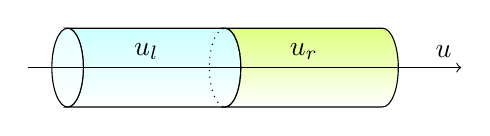
\begin{tikzpicture}
        \draw   [thin, shade,top color=cyan!20!white]  (0,-0.5) -- ++(2,0) 
    arc(-90:90:0.2 and 0.5) -- ++(-2,0) 
    arc(90:-90:0.2 and 0.5)--cycle;
        \draw   [thin, shade,top color=lime!50!white]  (2,-0.5) -- (4,-0.5) 
        arc(-90:90:0.2 and 0.5) -- ++(-2,0)
        arc(90:-90:0.2 and 0.5) --  cycle;
    

    \draw[thin, shade, top color=cyan!10!white] (0,0) ellipse(0.2 and 0.5);
    \draw[dotted] (2,0) ellipse(0.2 and 0.5);
        \node at (1,0.2) {$u_l$};
        \node at (3,0.2) {$u_r$};
        \draw[->] (-0.5,0) -- (5,0) node[anchor=south east] {$u$};
        \end{tikzpicture}
    \caption{Discontinuity}
    \label{Fig:riemann_tube}
    \end{center}
\end{wrapfigure}{}	 
	 
 Also, note that the conservation law is scale invariant. Which means that if we scale u with some parameter, it will not change the equation or the solution. $v(x,t) = u(\alpha x, \alpha t) \rightarrow \alpha u(t,x)$. Therefore we can introduce a scaling on $u(x,t) = \omega (x/t) $, $ \xi = x/t$. From a physical standpoint this makes sense, as we have either sharp discontinuities (shocks) from $u_l$ to $u_r$ or we can have solutions that smooth out from point $u_l$ to $u_r$. 

 \begin{equation*}
     \begin{split}
         0 &= u_t + f(u)_x = u_t + df(u)u_x \\
           &= \dot \omega( -\frac{x}{t^2}) + df( \omega) \dot \omega t^(-1) \\
           &= \frac{x}{t}(  df( \omega) \dot \omega - x/t \dot \omega )
     \end{split}
 \end{equation*}
 
 And we have the resulting equation 
 
 \begin{equation}
     df( \omega) \dot \omega =  \xi \dot \omega
 \end{equation}
 

\subsubsection{The scalar conservation law}
Let $u,f \in \mathbb{R}$. We can cancel $\dot \omega $, and if $f$ is (left) invertible (monotone, injevtive), we can find $u(x,t) = w(x/t) = (f')^{-1}(\frac{x}{t})$. 
To ensure this, we introduce the convex envelope $f_{\smile}(u) = \sup\{g(u) : g\leq f, \quad  g \quad \textit{convex on}\quad [u_l, u_r]\} $. We claim we have the solution for $u_r < u_l$:
	 
 \begin{equation}
     u(x,t) = \begin{cases} u_l, & \text{if $x < (f'_{\smile} )(u_l)t$}.\\
                            (f'_{\smile} )(x/t)t, & \text{if $(f'_{\smile} )(u_l)t$} < x < (f'_{\smile} )(u_r)t\\ 
                            u_r, & \text{if $x > (f'_{\smile} )(u_r)t$}. 
     \end{cases}
     \label{ScalarRiemannSol}
 \end{equation}
 
We can also construct the upper concave envelope, in case $u_rl > u_r$. Where $f_{\frown}(u) = \inf\{g(u) : g\leq f, \quad g \quad \textit{concave on} \quad  [u_r, u_l]\} $. And the principle is the same. 
    
   \begin{minipage}{\linewidth}
  \centering
  \begin{minipage}{0.45\linewidth}
      \begin{figure}[H]
          \includegraphics[clip, trim=2cm 14cm 2cm 2cm, width=0.65\textwidth]{Figures/ConservationLaws/convex_envelope.pdf}
          \caption{The convex envelope of $f$.}
      \end{figure}
  \end{minipage}
  \hspace{0.05\linewidth}
  \begin{minipage}{0.45\linewidth}
      \begin{figure}[H]
          \includegraphics[clip, trim=2cm 14cm 2cm 2cm, width=0.65\textwidth]{Figures/ConservationLaws/convex_derivative.pdf}
          \caption{The derivative of the convex envelope of $f$.}
      \end{figure}
  \end{minipage}
\end{minipage}  

 This has to be a weak solution as it satifies the equation and the traveling wave condition, and $f$ is never below $f_{\smile}$. Notice we have the same deriavte at $u_2$ and $u_3$ so Rankine-Hugoniot is still satified. 
 

\begin{theorem}
The initial value problem
\begin{equation}
    u_t + f(u)_x = 0,  \quad u|_{t = 0 } = \begin{cases} u_l, & \text{if $x \leq 0$}.\\ u_r, & \text{if $x>0$} 
 \end{cases}
\end{equation}
 with a flux function $f(u)$ such that $f_{\smile,\frown} \neq f$ on finitely many intervals, alternating with intervals where they coincide, has a weak solution given by the equation \ref{ScalarRiemannSol} if $u_l > u_r$. And if $u_r > u_l$, we construct a concave envelope.  
\label{RP_Kruzkov_sol}
\end{theorem}

For the proof of this theorem we need the Kruzkov entropy condition. The proof, a long with the Kruzkov theory, will be given in section \ref{The Kruzkov entropy}, about Kruzkov entropy. 


% ---------------------------------------------
% ---------------------------------------------

\subsubsection{The conservation law for systems }
Let $u, f \in \mathbb{R}^n$ and thus $\partial f(u)$ is the non-linear Jacobian matrix of the system. However, in this case we cannot cancel $ \dot \omega$ as in the scalar case, and we are left with an eigenvalue problem. We will assume that the Jacobian $df(u)$ has $n$ real eigenvalues 

\begin{equation}
    df(u)\boldsymbol{r_j}(u) = \lambda_j(u)\boldsymbol{r_j}(u), \quad \lambda_j(u) \in \mathbb{R}, \quad j = 1, \dots, n 
    \label{Eig.val problem}
\end{equation}


If the eigenvalues $\lambda_1 \leq \lambda_2 \leq \dots \leq \lambda_n $ are real, we have a hyperbolic system. If the eigenvalues are distinct, the system is strictly hyperbolic. 

From the assumptions of the Riemann problem, and the assumptions on the flux function we have the following 
\begin{equation*}
    \begin{cases}
    \omega( \lambda_j( u_l) ) = u_l \\
    \omega( \lambda_j( u_r) ) = u_r \\
    \\
    \dot \omega( \xi ) = \boldsymbol{r_j}( \omega(\xi)) \\
    \lambda_j (\omega(\xi)) = \xi \\
    \end{cases}
\end{equation*}

From the assumptions above, for a fixed time $t$ the function $\omega(x/t)$ will connect $u_l$ to $u_r$. For the case $u_l < u_r$, $\xi$ must be increasing, thus $\lambda_j( \omega(x/t)$ must be increasing. Hence, we have the rarefaction solution 

\begin{equation}
     u(x,t) = \begin{cases} u_l, & \text{if $x < \lambda_j(u_l)t$}.\\
                            \omega(x/t), & \text{if $ \lambda_j(u_l)t$} < x <  \lambda_j(u_r)t\\ 
                            u_r, & \text{if $x >  \lambda_j(u_r)t$}. 
     \end{cases}
     \label{SystemRiemannSol}
 \end{equation}

We investigate further the last assumption

\begin{align*}
    \frac{d}{d\xi} \xi = \frac{d}{d\xi} \lambda_j( \omega \xi)) \\
    1 = \nabla \lambda_j \cdot \dot \omega (\xi) \\
\end{align*}

However, if we have constant velocities $\xi, \lambda_j$ this will not hold. Thus, we have the following

\begin{align}
    \nabla \lambda_j \cdot r_j = 1, \quad \text{Genuinely nonlinear } \\
    \nabla \lambda_j \cdot r_j = 0, \quad \text{Linearly degenerate }
\end{align}

Furthermore, looking at the second to last assumption $\dot \omega( \xi ) = \boldsymbol{r_j}( \omega(\xi))$. The integral (rarefaction) curves in the $u$ plane , using the initial condition $\omega (\lambda_j (u_l)) = u_l$, are denoted $R_j(u_l)$. Similarly, we can do this for $u_r$.

Investigating the linearly degenerate case, we want to create a phase path of the eigenvectorfield. In this case, $\lambda$ is constant along the integral curve, and we have 

\begin{align*}
    \frac{d}{d\xi} f(u) = df(u) \dot u = df(u) \cdot r_j = \lambda_j \cdot r_j = \lambda_j \dot u \\
     \frac{d}{d\xi} \lambda = \nabla \lambda_j \cdot r_j = 0 \\
     \frac{d}{d\xi} f(u) =  \frac{d}{d\xi}( \lambda_j u ) \\
     f(u) = \lambda_j u 
\end{align*}

The Rankine-Hugoniot relation is retrieved. We call path in the phase plane the contact discontinuity, and the rarefaction and the shock curves must necessarily be the same in this case. Also, the weak solution is satisfied. 

The obvious extension is to define the shock curves in the phase plane. Now assume $u_l$ is fixed, and we consider all possible states $u$ that satisfy the Rankine-Hugoniot relation. We call the trajectories in the phase plane the Hugoniot Locus:
\begin{equation}
    \label{Hugoniot_locus}
    H(u_l) := \{ u : \exists s\in \mathbb{R} \quad \text{such that} \quad s[u] = [f] \}
\end{equation}

However, the system $ \mathcal{H} := s[u] - [f] = 0 $ has $n$ equations, so we have $n+1$ unknowns in our case. Using the implicit function theorem we can prove that in a neighbourhood of $u_l$ we have $n$ unique differentiable solutions, only requiring that $d \mathcal{H}$ is non-singular. \todo{include proof?}
 


\subsection{Entropy Conditions}

We know have $n$ rarefaction- and shock curves around $u_l$. We will now investigate which of these lead to permissable solutions of both scalar and systems of conservarion laws. We investigate the viscous regularization equation, for $\epsilon > 0 $

\begin{equation}
    u_t + f(u)_x = \epsilon u_{xx}
    \label{Viscous_reg}
\end{equation}

which is well-posed. And if we let $\epsilon \to 0$ we arrive at the limitcase of the conservation law. We look for traveling wave solutions of the form $u(x,t) = U(\frac{x-st}{\epsilon}), \quad \xi = \frac{x-st}{\epsilon}$. Differentiation with respect to xi, we get the ordinary differential equation

\begin{equation*}
	    \begin{split}
	        \frac{-s}{\epsilon} \dot U + \frac{1}{\epsilon} f'(U) \dot U = \frac{\epsilon}{\epsilon^2} \ddot U \\
	        \dot U = -sU + f(U) + A \\
	    \end{split}
\end{equation*}

\begin{align*}
    \xi \rightarrow -\infty, \dot U \rightarrow 0: \quad \dot U = f(U) - f(u_l) - s(U-u_l) \\
    \xi \rightarrow \infty, \dot U \rightarrow 0: \quad  \dot U = f(U) - f(u_r) - s(U-u_r)
    \label{travelling wave}
\end{align*}

This yields the travelling wave relation: 
\begin{equation*}
    s|k-u_l| < sgn(u-k)(f(k)-f(u_l)), \quad u_l < k < u_r
\end{equation*}

\subsubsection{The Lax entropy}\label{The Lax entropy}

In the systems case, $\dot U = f(U) - f(u_l) - s(U-u_l)$ will give the flow in the eigenvectorspace, and determines wheter or not we can connect $u_l$ to $u_r$. 

For the systems case, the eigenvalues in the critical point determines the behaviour of the eigenvectorfield. In our (real) case, we have the following possibilites, $\boldsymbol{\lambda} > 0 $ source, $\boldsymbol{\lambda} < 0 $ sink, $\lambda_i < 0 < \lambda_j $ saddle. \cite{VerhulstFerdinand1990NDEa}
It is clear that for there to exist an orbit from $u_l$ to $u_r$, $u_l$ cannot be a pure sink, and $u_r$ cannot be a pure source. This means we go from $9$ different combinations, down to $4$, and can be seen in the Figure below. 

% ---- TIKZ FIGURE -----
\vspace{6pt}
\begin{minipage}{.2\textwidth}
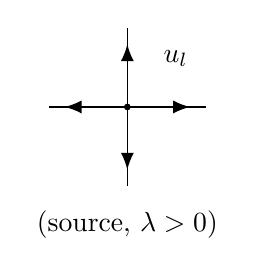
\begin{tikzpicture}
[decoration={markings, 
        mark= at position 0.8 with {\arrow[line width=0.4mm]{latex}} }
] 
\draw[postaction = {decorate}] (1,0) -- (0,0); 
\draw[postaction = {decorate}] (1,0) -- (2,0); 
\draw[postaction = {decorate}] (1,0) -- (1,1);
\draw[postaction = {decorate}] (1,0) -- (1,-1);
\filldraw[black] (1,0) circle (1pt) ;
\node at (2, 1,1) {$u_l$};
\node at (1,-1.5) {(source, $\lambda > 0$)};
\end{tikzpicture}
\end{minipage}
\begin{minipage}{.2\textwidth}
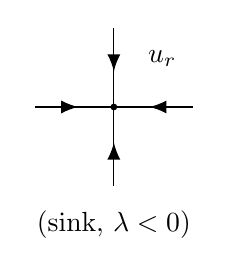
\begin{tikzpicture}
[decoration={markings, 
        mark= at position 0.55 with {\arrow[line width=0.4mm]{latex}} }
] 
\draw[postaction = {decorate}] (0,0) -- (1,0); 
\draw[postaction = {decorate}] (2,0) -- (1,0); 
\draw[postaction = {decorate}] (1,1) -- (1,0);
\draw[postaction = {decorate}] (1,-1) -- (1,0);
\filldraw[black] (1,0) circle (1pt) ;
\node at (2, 1,1) {$u_r$};
\node at (1,-1.5) {(sink, $\lambda < 0$)};
\end{tikzpicture}
\end{minipage}
\quad
\begin{minipage}{.2\textwidth}
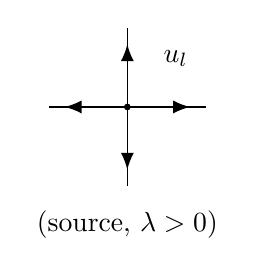
\begin{tikzpicture}
[decoration={markings, 
        mark= at position 0.8 with {\arrow[line width=0.4mm]{latex}} }
] 
\draw[postaction = {decorate}] (1,0) -- (0,0); 
\draw[postaction = {decorate}] (1,0) -- (2,0); 
\draw[postaction = {decorate}] (1,0) -- (1,1);
\draw[postaction = {decorate}] (1,0) -- (1,-1);
\filldraw[black] (1,0) circle (1pt) ;
\node at (2, 1,1) {$u_l$};
\node at (1,-1.5) {(source, $\lambda > 0$)};
\end{tikzpicture}
\end{minipage}
\begin{minipage}{.2\textwidth}
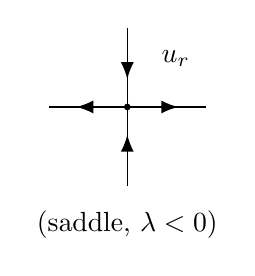
\begin{tikzpicture}
[decoration={markings, 
        mark= at position 0.65 with {\arrow[line width=0.4mm]{latex}} }
] 

\draw[postaction = {decorate}] (1,0) -- (0,0); 
\draw[postaction = {decorate}] (1,0) -- (2,0); 
\draw[postaction = {decorate}] (1,1) -- (1,0);
\draw[postaction = {decorate}] (1,-1) -- (1,0);
\filldraw[black] (1,0) circle (1pt) ;
\node at (2, 1,1) {$u_r$};
\node at (1,-1.5) {(saddle, $\lambda < 0$)};
\end{tikzpicture}
\end{minipage}

\begin{minipage}{.2\textwidth}
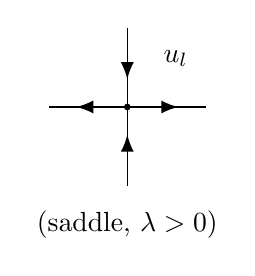
\begin{tikzpicture}
[decoration={markings, 
        mark= at position 0.65 with {\arrow[line width=0.4mm]{latex}} }
] 
\draw[postaction = {decorate}] (1,0) -- (0,0); 
\draw[postaction = {decorate}] (1,0) -- (2,0); 
\draw[postaction = {decorate}] (1,1) -- (1,0);
\draw[postaction = {decorate}] (1,-1) -- (1,0);
\filldraw[black] (1,0) circle (1pt) ;
\node at (2, 1,1) {$u_l$};
\node at (1,-1.5) {(saddle, $\lambda > 0$)};
\end{tikzpicture}
\end{minipage}
\begin{minipage}{.2\textwidth}
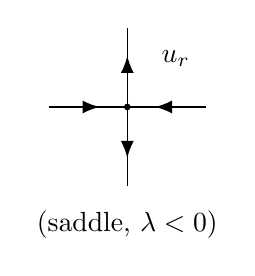
\begin{tikzpicture}
[decoration={markings, 
        mark= at position 0.65 with {\arrow[line width=0.4mm]{latex}} }
] 
\draw[postaction = {decorate}] (0,0) -- (1,0); 
\draw[postaction = {decorate}] (2,0) -- (1,0); 
\draw[postaction = {decorate}] (1,0) -- (1,1);
\draw[postaction = {decorate}] (1,0) -- (1,-1);
\filldraw[black] (1,0) circle (1pt) ;
\node at (2, 1,1) {$u_r$};
\node at (1,-1.5) {(saddle, $\lambda < 0$)};
\end{tikzpicture}
\end{minipage}
\quad
\begin{minipage}{.2\textwidth}
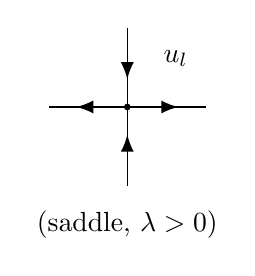
\begin{tikzpicture}
[decoration={markings, 
        mark= at position 0.65 with {\arrow[line width=0.4mm]{latex}} }
] 
\draw[postaction = {decorate}] (1,0) -- (0,0); 
\draw[postaction = {decorate}] (1,0) -- (2,0); 
\draw[postaction = {decorate}] (1,1) -- (1,0);
\draw[postaction = {decorate}] (1,-1) -- (1,0);
\filldraw[black] (1,0) circle (1pt) ;
\node at (2, 1,1) {$u_l$};
\node at (1,-1.5) {(saddle, $\lambda > 0$)};
\end{tikzpicture}
\end{minipage}
\begin{minipage}{.2\textwidth}
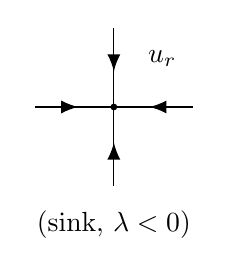
\begin{tikzpicture}
[decoration={markings, 
        mark= at position 0.55 with {\arrow[line width=0.4mm]{latex}} }
] 
\draw[postaction = {decorate}] (0,0) -- (1,0); 
\draw[postaction = {decorate}] (2,0) -- (1,0); 
\draw[postaction = {decorate}] (1,1) -- (1,0);
\draw[postaction = {decorate}] (1,-1) -- (1,0);
\filldraw[black] (1,0) circle (1pt) ;
\node at (2, 1,1) {$u_r$};
\node at (1,-1.5) {(sink, $\lambda < 0$)};
\end{tikzpicture}
\end{minipage}
\vspace{6pt}

In $n$ dimensions, we can have a combination of positive of negative eigenvalues.  When examining the possible flows in the eigenvectorfield, it is clear that at least one eigenvalue at $u_l$ needs to be larger than the one in $u_l$. for there to be an orbit connecting them. We summarize this result into Lax' entropy condition

\begin{equation}
    \lambda_{j-1}(u_r) < s < \lambda_{j}(u_r), \quad \text{for orbits $u_l$ to $u_r$}
\end{equation}

\begin{definition}[Lax j-shock]
We say that a shock is a Lax j-shock if the speed satisfies the Rankine Hugoniot relation and 
\begin{align*}
    \lambda_{j-1}(u_l) < s < \lambda_{j}(u_l) \\
    \lambda_{j}(u_r) < s < \lambda_{j+1}(u_r)
\end{align*}
\end{definition}


\subsubsection{The Kruzkov entropy}\label{The Kruzkov entropy}
Let $\eta = \eta(u)$ be a smooth convex function, and $\phi > 0$ our usual test function, $\phi \in C_0^\infty(\mathbb{R} \times (0, \infty))$ with compact support away from the x-axis. We will now investigate the case

\begin{align}
   0 &= \int_0^T \int_{\mathbb{R}} (u_t + f(u)_x - \epsilon u_{xx}) \eta' \phi dxdt \\
   &= \int_0^T \int_{\mathbb{R}} \underbrace{\eta'u_t}_{\eta_t}  \phi dx dt + \int_0^T \int_{\mathbb{R}} \underbrace{f'(u)\eta'}_{q'} u_x \phi dxdt - \epsilon \int_0^T \int_{\mathbb{R}} \underbrace{ u_{xx}\eta'}_{(\eta'u_x)_x - \eta''u_x^2}\phi dxdt \\
   &= \int_0^T \int_{\mathbb{R}}  \eta \phi_t dx dt + \int_0^T \int_{\mathbb{R}} q \phi_x dxdt  - \epsilon \int_0^T \int_{\mathbb{R}} \underbrace{ \eta'' (u_x)^2 \phi}_{ \geq 0} dxdt +  \epsilon \int_0^T \int_{\mathbb{R}} \eta \phi_{xx} dxdt \\
   & \leq \int_0^T \int_{\mathbb{R}} \bigg ( \eta \phi_t + q\phi_x + \epsilon \eta \phi_{xx} \bigg ) dx dt 
\end{align}    

\todo{fill in some details from the proof above}
Letting $\epsilon$ go to zero

\begin{equation}
    \int_0^T \int_{\mathbb{R}}( \eta \phi_t + q \phi_x)dxdt \geq 0
    \label{Kruzkov_distributions}
\end{equation}

We get the Kružkov entropy condition, in the sense of distributions. 

\begin{wrapfigure}[13]{L}{0.5\textwidth}
    \begin{center}
        \includegraphics[valign = c,clip, trim=2cm 18cm 2cm 2cm, width=0.4\textwidth]{Figures/ConservationLaws/convex.pdf}
    \caption{Convex function}
    \label{Fig:convex}
    \end{center}
\end{wrapfigure}{}
	  
Now, let us examine a generic convex function $\eta_\delta = \sqrt{(u-k)^2 + \delta^2}$, $\delta > 0 $.  Note that  $\lim_{\delta \to 0} = |u-k|$. And recall from above that we used $q' = \eta' f'(u)$, integrating we have

\begin{equation}
    q(u) = \int_k^u \eta' f'(v) dv = sgn(u-k)(f(u) - f(k))
\end{equation}

And we get the \textit{Kružkov entropy} condition

\begin{equation}
    \iint ( |u-k|\phi_t + sgn(u-k)( f(u) - f(k))\phi_x) dx dt \geq 0
    \label{Kruzkov}
\end{equation}

If $u$ satisfies this, its called a Kružkov entropy solution for all $k$ in $\mathbb{R}$.  If we let k be less than either $u_l$ or $u_r$ we retrieve Rankine-Hugoniot. And let $k$ be greater than $u_l$ or $u_r$ we also retrieve Rankine Hugoniot. Which implies that Kružkov is a weak solution. Also, note that we can easily extend this to include the initial condition. This would have given us an extra term $- \int_\mathbb{R} \eta \phi |_{t= 0}^{t = T} dx$

 We can approximate eta as a sum of piecewice convex linear functions. Such that any convex piecewise lin. function converges to eta in $L^{inf}$. This means that Kružkov holds for all convex functions. \todo{Add proof of convex functions}

We can show that Theorem \ref{RP_Kruzkov_sol} satisfies the Kruzkov entropy condition \ref{Kruzkov}. 
To complete the proof of \ref{RP_Kruzkov_sol}, we need to show that \ref{ScalarRiemannSol} indeed satistfies the Kruzkov entropy. 

The solution u consists of a finite number of discontinuities (shocks), seperated by wedges, and the continous parts are rarefaction waves. The solution of the Riemann problem consists of a finite sequence of rarefaction waves alternating with shocks.

\begin{equation}
    \begin{split}
        \int_0^T \int_{\mathbb{R}} \big ( \eta \phi_t + q\phi_x\big ) dx dt &=  \sum_i \int \int_{\Omega_i}(\eta_i\phi_t + q_i\phi_x)dxdt \\
        &=  \sum_i \int \int_{\Omega_i}(\eta_i\phi_t + q_i\phi_x + \underbrace{(\eta_t + q_x)}_{=0}\phi )dxdt \\ &= \sum_i\int \int_{\Omega_i}( (\eta_i \phi)_t + (q_i \phi)_x )dxdt 
    \end{split}
\end{equation}

\begin{wrapfigure}[14]{R}{0.5\textwidth}
    \begin{center}
        \includegraphics[valign = c,clip, trim=8cm 25.5cm 2cm 2.5cm, width=1.2\textwidth]{Figures/ConservationLaws/discrete_domain.pdf}
    \caption{Discrete domain}
    \label{Fig:discrete_domain}
    \end{center}
\end{wrapfigure}{}	 

Note that Theorem 2.2 does not require the flux function f to be differentiable. Assume now that the flux function is a polygon, i.e., that $f$ is continuous and piece- wise linear on a finite number of intervals. Thus $f'$ will then be a step function taking a finite number of values.    This means that the envelopes also will be stepfunctions. If the initial states in a Riemann problem are breakpoints, then the entire solution will take values in the set of breakpoints.



\begin{equation}
\begin{split}
    \int_0^T \int_{\mathbb{R}} \big ( \eta \phi_t + q\phi_x\big ) dx dt &= \sum_i \int\int_{\partial \Omega_i}( -(\eta_i \phi)dt + (q_i \phi)dx )) \\
    &= \sum_i \int_{\partial \Omega_i} \phi(q_i,\eta_i) \cdot \Vec{n} ds \\
    &= \int_{\mathbb{R}} \eta \phi \bigg|_{t=0}^{t=T} dx + \sum_i \int_0^T \underbrace{\phi(\sigma_it,t)}_{\geq 0} \underbrace{\bigg( \sigma_i(\overline{\eta_i} - \underline{\eta_i}) -( \overline{q_i} -\underline{q_i}) \bigg )}_{\geq 0 \quad \text{Travelling Wave} }dt \\
    & \geq  \int_{\mathbb{R}} \eta \phi \bigg|_{t=0}^{t=T} dx
\end{split}
\end{equation}

Which concludes that the Riemann solution above indeed satisfies the Kruzkov entropy if $u_l < u_r$.

It can also be shown that Theorem \ref{RP_Kruzkov_sol} also holds for piecewise linear flux functions.


\begin{definition}[Total Variation]
Let $J \subseteq \mathbb{R}$ and $w : J \to \mathbb{R}$. The total variation of $w$ is defined by
\begin{equation}
    TV(w) = \sup \bigg \{ \sum_{j=1}^{N} |w(x_j)-w(x_{j-1})| \bigg \} 
\end{equation}
\end{definition}

\begin{definition}
We say that the function $w : J \to \mathbb{R}$ has bounded total variation if $TV(w) < \infty $. We denote BV(J) the set of all real functions  $w : J \to \mathbb{R}$ with bounded total variation. 
\end{definition}



%\begin{theorem}
%Let $u_0 \in L^1$ be a function of bounded total %variation, and $f(u)$ be a piecewise twice %continously differentiable function. Then there %exists a unique weak solution $u = u(x,t)$ to the %initial value problem
%\begin{equation*}
%    u_t + f(u)_x = 0, \quad u(x,0) = u_0(x)
%\end{equation*}
%which also satisfies the Kruzkov entropy condition %\ref{Kruzkov}. Furthermore, if $v_0$ is another %function in $BV \cap L^1(\mathbb{R}$, $g(v)$ is a %piecewise twice continously differentiable %function, and $v$ is the unique Kruzkov entropy %solution to 
%\begin{equation*}
%    v_t + g(v)_x = 0, \quad v(x,0) = v_0(x)
%\end{equation*}
%then
%\begin{equation}
%    ||u(\cdot,t) - v(\cdot, t)||_{L^1} + t \min %\{TV(u_0), TV(v_0)\}||f-g||_{Lip}
%\end{equation}

%\label{The_ultimate_result_scalar}
%\end{theorem}

%A proof of this result can be found in chapter 2.4 %in  \cite{HoldenH.Helge2015Ftfh}. 


\subsection{The solution of the Riemann problem}
We will now generalize the previous results, assuming without loss of generality $u_l$ to be fixed. Then, show $u_l$ can be connected to $u_r$ using a series of rarefaction waves and shock waves. 

For the scalar case, note that Theorem \ref{RP_Kruzkov_sol} does not require $f$ to be differentiable. Thus, now assume $f$ to be a step-function, a continous and piecewise linear on a finite number of intervals. Then, also $f_{\smile}'$ and $f_{\frown}'$ will be stepfunctions, as will their inverses. Furthermore, assume $u_l = u_0 < u_1 < \dots < u_n = u_r$, and $f_\smile$ has breakpoints in some subsets of this. Thus we have discontinuities given by 

\begin{corollary}
Assume $f$ is a continous piecewise linear function $f: [-K, K] \rightarrow \mathbb{R}$ for some constant $K$. Denote the brakpoints of $f$ by $-K = u_0 < u_1 < \dots < u_{n-1} < u_n = K$. Then the Riemann problem 
\begin{equation}
    u_t + f(u)_x = 0, u(x, 0) = \quad \begin{cases} u_j, \text{for} x < 0, \\ u_k \text{for} x \geq 0 \end{cases}
\end{equation}
has a piecewise constant solution. 
If $u_j < u_k$, let $u_j = v_1 < \dots <v_m = u_k$ denote the brakpoints of $f_\smile$, and if $u_j > u_k$, let $u_k = v_m < \dots <v_1 = u_j$ denote the brakpoints of $f_\frown$. The weak solution of the Riemann problem is given by 

\begin{equation}
    u(x,t ) = \begin{cases}
    v_1, \quad \text{for} \quad x \leq s_1t, \\
    v_2, \quad \text{for} \quad s_1t \leq s_2 t\\
    \vdots \\
    v_i, \quad \text{for} \quad s_{i-1}t \leq s_i t\\
    \vdots \\
    v_m \quad \text{for} \quad s_{m-1}t < x
    \end{cases}
\end{equation}

where the speeds $s_i$ are computed from the derivative of the envelope, 
\begin{equation*}
    s_i = \frac{f(v_{i+1}) - f(v_i) } {v_{i+1} - v_i }
\end{equation*}

Furthermore, for a fixed time $t$, the solution is monotone in the $x$ variable. 
\begin{equation*}
    || u(\cdot, t) - u_0 ||_{L^1} \leq t||f||_{Lip} |u_j - u_k|
\end{equation*}
\end{corollary}


\section{A traffic model with phase transitions}
%\subsection{Phase Transition Model}
A phase transition model for traffic flow was proposed by Colombo in $2002$ \cite{Colombo2003}. The model is a coupled scalar conservation law with a $2 \times 2$ system of conservation laws, where the assumption is that traffic consists of two different \textit{phases}, a free flow phase and a congested flow phase. The argument for this model is deep qualitative difference between the phases, and thus cannot be modelled solely by a single equation. The coupling is achieved via a free boundary, which means that the interface between the two states is dynamically controlled by the system. A typical free boundary model is the melting of ice into liquid, where the boundary is controlled by the heat equation. 

Colombo suggests using the classical LWR model for the free phase. In this phase, the assumption is that the density $\rho$ is determined by the speed of the cars, $v(\rho)$. However, as the car density increases, the assumption that the speed is a function only on the density is no longer acceptable, and the density-flow points are scattered on a cloud rather than along a line. We denote this phase as the congested flow. 
%Imagine driving on a motorway, when there are few cars on the road you are free to change your velocity as you please. If you break, the car behind you will approach and the effect on the system will be an increase in density. If we instead choose to speed up, the distance between cars will increase and we have a lower density. However, when there many cars on the motorway, we are forced to reduce our speed to avoid collisions. And for a fixed density, we are allowed different speeds. A car jam can move at several different speeds, depending on factors like speed limit, the road it self, and the individual drivers. Also, different drivers tend to move at different speeds in the same velocities. We always have these few drivers who let a large portion of the road clear before picking up speed.  
Colombo proposes the following model for traffic flow: 

\begin{align}
    & \text{Free flow:}  (\rho, q) \in \Omega_f, \quad \quad \quad \text{Congested flow:} (\rho, q) \in \Omega_c, \\
    & \rho_t + (\rho v )_x = 0, \quad \quad   \quad \quad \quad \quad 
    \begin{cases}
    \rho_t + (\rho v )_x = 0 , \\
    q_t + ((q-Q)v)_x = 0 
    \end{cases} \\
    & v = v_f(\rho) = \big(1- \frac{\rho}{R}\big)V \quad \quad \quad v = v_c(\rho,q) = \big(1 - \frac{\rho}{R}\big)\frac{q}{\rho}
    \label{Eq:phase-transition}
\end{align}

Here we have the density $\rho$ and velocity $v$ as independent variables. The variable $q$ is the weighted flow, where the original motivation stems from gas dynamics, where it describes linear momentum. The two phases have different speed laws, but the maximal car density $R$, the maximal speed $V$ and the wide jam parameter $Q$ are all global and constant for the model. 

Note that the road is spatially and temporally translation invariant,  as none of the expressions depends explicitly on space or time. Thus, the model is not able to predict when or where phase transitions may appear. However, we are able to predict under which circumstances a queue forms, given the left and right states. The wave curve families, rarefaction and Hugoniot curves, will be invariant under a uniform linear scaling transformation. 
Wave curve families will be invariant under these transformations, in this case a different scaling of $\rho$ and $q$. This is useful; instead of looking at a  large family of curves, we choose one representative sample of the family and understand this, and in principle, we have understood the whole system, as the rest of the curves are just scaled versions of the representative. As a consequence of translation invariance, Colombo suggests that if initial data is contained on a single phase, it will remain in the same phase for all times. It is natural for us to first investigate the Riemann problem with initial data in the free phase, then look at the Riemann problem for the congested phase, and lastly combining the two and looking at initial data in different phases where we will experience a phase transition.

First, Colombo states a few necessary criteria in order to make the traffic flow realistic:
\begin{enumerate}
    \item The driver reacts to what is seen in front of the car, no information travels faster than cars.
    \item We cannot have a negative car density, and cars cannot travel backwards, $\rho, q \geq 0$.
    \item We have a maximal car density $R$, so that whenever a queue is formed the maximal density is reached. 
    \item Below this maximal car density, no car may stop. We are driving on a motorway until a something happens. 
    \item When moving at \textit{high} car densities and speeds accelerating produce rarefaction, and breaking produce shocks. At low car density and speeds, the opposite occurs \cite{Colombo2002}. 
\end{enumerate} The criteria above will be investigated as we go through the solution of the Riemann problem for the model. 

\subsection{The Riemann Problem for Free Phase}\label{RPFreePh}
We start off by analysing the properties of the free phase, and we will at the end give the full solution for the Riemann problem for the free phase. We examine the flux function as a function of the density in a fundamental diagram. 
\begin{figure} \centering 
\begin{minipage}{.35\textwidth}
\begin{tikzpicture}
\draw[->] (0,-0.2) -- (0,2.5);
\draw[->] (-0.2,0) -- (2.5,0);
\draw[->][magenta!70] (0,2) -- (0.8,1.2) node[anchor = south west] {$V_f$};
\draw[>-][black!30] (2,0) -- (1.2,0.8) node[anchor = south west] {$V_c$};
\draw[black!10] (2,0) -- (0.8,1.2);
%\node[magenta!70] at (1.3,1.1) {$V_f$};
\node at (2, -0.2) {$R$};
\node at (-0.2, 2) {$V$};
\node at (2.6, -0.2) {$\rho$};
\node at (-0.2, 2.6) {$v$};
\end{tikzpicture}
\caption{The velocity function.}
\label{Fig:Velocity function}
\end{minipage}
\begin{minipage}{.35\textwidth}
\begin{tikzpicture}
\draw[->] (0,-0.2) -- (0,2);
\draw[->] (-0.2,0) -- (2.5,0);
\draw[cyan!50]  plot [smooth, tension = 1.5] coordinates { (0,0) (1,1) (2,0)};
\node at (2, -0.2) {$R$};
%\node at (-0.2, 2) {$V$};
\node at (2.6, -0.2) {$\rho $};
\node at (-0.2, 2.1) {$\rho v$};
\end{tikzpicture}
\caption{The flux function, or the velocity function in the $(\rho, \rho v)$-plane.}
\label{Fig:Flux function}
\end{minipage}
\end{figure}

As soon as $\rho$ crosses a certain threshold, we no longer regard $v$ as a function only on density, but also momentum. We call this threshold velocity, the constant $V_f$, see Figure \ref{Fig:Velocity function}. So as $\rho \nearrow R$, and thus $v \searrow V_f$, which means $V > V_f $, see Figure \ref{Fig:Velocity function}. Also, note that the flux function is concave in the $(\rho, \rho v)$-plane, see Figure \ref{Fig:Flux function}, which means we are able to invert the flux function without using convex envelopes. We have the characteristic speed $df(\rho) = V(1- \frac{2\rho}{R})$ and its clear we have a strictly hyperbolic system, and no information travels faster than the cars. We have achieved criteria $1.$ for realistic traffic flow, for the free phase. This leads us to define the domain for the free phase

\begin{equation}
    \Omega_f = \{(\rho, q) \in [0, \mathbb{R}] \times [0, \infty) : v_f(\rho) \geq V_f, q= \rho V \}
    \label{Domain free ph}
\end{equation}

Riemann problem has the following solution in the free phase, $(\rho_l, \rho_r) \in \Omega_f$
\begin{align*}
    \rho_t + (\rho v)_x = 0,\quad  \rho(0,x) = \begin{cases} 
    \rho_l , \quad x < 0 \\
    \rho_r, \quad x \geq 0 
    \end{cases}
\end{align*}

\paragraph{Shock solution.} If $\rho_l < \rho_r$, the entropy-admissible solution is given by the shock wave, as $f \in C^2$ and $f$ is strictly concave and thus $f'(\rho_l) > f'(\rho_r) $. The shock speed given by the Rankine-Hugoniot condition
\begin{align*}
    & \rho(x,t) = \begin{cases}
    \rho_l, \quad x < s t \\
    \rho_r, \quad x > s t
    \end{cases} 
    \quad \quad s = \frac{f(\rho_r) - f(\rho_l)}{\rho_r - \rho_l} = \frac{\rho_r v_f(\rho_r) -\rho_l v_f(\rho_l)}{\rho_r - \rho_l}
\end{align*}

\paragraph{Rarefaction solution.} If $\rho_l > \rho_r$, then $f'(\rho_l) < f'(\rho_r) $ so the entropy-admissible solution is given by a rarefaction wave.
\begin{align*}
    & \rho(x,t) = \begin{cases}
    \rho_l, \quad x < f'(\rho_l)t \\
    (f')^{-1}(x/t),  \quad  f'(\rho_l)t < x < f'(\rho_r)t \\
     \rho_r, \quad x > f'(\rho_r)t
    \end{cases} \\
    & f'(\rho) = V(1-\frac{2 \rho}{R}V) , \quad  (f')^{-1}(\xi) = \frac{R}{2}(1-\frac{\xi}{V}) 
\end{align*}

We conclude this solution of the phase transition model if initial data $\rho_l, \rho_r \in \Omega_f$.

\begin{figure} \centering
\begin{minipage}{.3\textwidth}
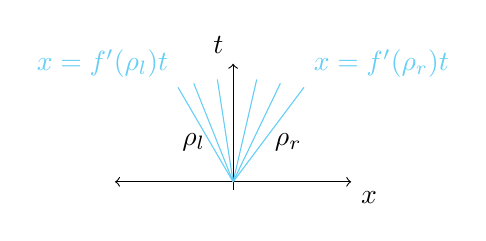
\begin{tikzpicture}
% coord.
\draw[<->] (-1.5,0) -- (1.5,0) node[anchor= north west] {$x$};
\draw[->] (0,-0.1) -- (0,1.5) node[anchor=south east] {$t$};
% rarefaction
\draw[color=cyan!60!white] (0,0) -- (0.9,1.2) node[anchor= south west] {$x = f'(\rho_r)t$};
\draw[color=cyan!60!white] (0,0) -- (0.6,1.25);
\draw[color=cyan!60!white] (0,0) -- (0.3,1.3);
\draw[color=cyan!60!white] (0,0) -- (-0.2,1.3);
\draw[color=cyan!60!white] (0,0) -- (-0.5,1.25);
\draw[color=cyan!60!white] (0,0) -- (-0.7,1.2) node[anchor= south east] {$x = f'(\rho_l)t$};
\node at (-0.5, 0.5) {$\rho_l$};
\node at (0.7, 0.5) {$\rho_r$};
\end{tikzpicture}
\caption{The solution to the Riemann problem, $\rho_l < \rho_r$.}
\label{Fig: SolRP_raref_disc}
\end{minipage}
\quad \quad \quad \quad \quad \quad \quad \quad
\begin{minipage}{.3\textwidth}
\begin{tikzpicture}
\draw[<->] (-1.5,0) -- (1.5,0) node[anchor= north west] {$x$};
\draw[->] (0,-0.1) -- (0,1.5) node[anchor=south east] {$t$};
\draw[color=cyan!90!white] (0,0) -- (0.9,1.2) node[anchor= south west] {$x = st$};
\node at (-0.5, 0.5) {$\rho_l$};
\node at (0.7, 0.5) {$\rho_r$};
\end{tikzpicture}
\caption{The solution to the Riemann problem, $\rho_l < \rho_r$.}
\label{Fig: SolRP_shock_disc}
\end{minipage}
\end{figure}


\subsection{The Riemann Problem for the Congested phase}\label{RPCongPh}

When the velocity $v$ decreases and reaches the constant threshold $V_c$ see Figure \ref{Fig:Velocity function}, the traffic enters the congested phase . Now we have the relation $ V > V_f > V_c $, and we define the congested phase

\begin{equation}
    \Omega_c = \Bigg\{(\rho, q) \in [0, \mathbb{R}] \times [0, \infty) : v_c(\rho, q) \leq V_c, \frac{q-Q}{\rho} \in \Bigg[\frac{Q_1 - Q}{R}, \frac{Q_2 - Q}{R} \Bigg]  \Bigg\}
    \label{Domain congested ph}
\end{equation}

\begin{wrapfigure}[10]{L}{0.3\textwidth}
    \begin{center}
        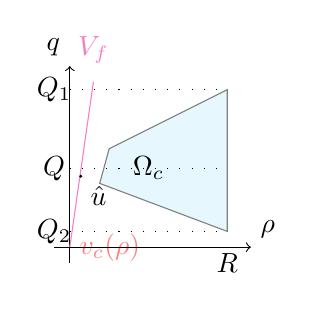
\begin{tikzpicture}
        % coordinates
        \draw[->] (0,-0.2) -- (0,2.3) node[anchor=south east] {$q$};
        \draw[red!50, domain=0:0.7]  plot[id=x] function{x*(3*x+1)}  node[right] {$v_c(\rho)$};
        \draw[magenta!50] (0,0) -- (0.3,2.1);
        \node[magenta!50] at (0.3,2.5) {$V_f$};
        \filldraw[black] (0.14,0.9) circle (0.3pt) node[anchor = north west]{$\hat u$} ;
         \filldraw[fill=cyan!10!white, draw=black!50] plot [tension = 1] coordinates { (0.5,1.25) (2,2) (2,0.2) (0.38, 0.81) (0.5,1.25)};
         \node at (1,1) {$\Omega_c$};
         \draw[->] (-0.2,0) -- (2.3,0) node[anchor=south west] {$\rho$};
        \node at (2,-0.2) {$R$};
         \node at (-0.2,2) {$Q_1$};
         \node at (-0.2,0.2) {$Q_2$};
         \node at (-0.2,1) {$Q$};
         \draw[loosely dotted] (0,1) -- (2,1);
         \draw[loosely dotted] (0,2) -- (2,2);
         \draw[loosely dotted] (0,0.2) -- (2,0.2);
       \end{tikzpicture}
    \caption{Domain  $\Omega_c$}
    \label{fig:ConservationLaws/I}
    \end{center}
\end{wrapfigure}{}

Where $Q_1$ and $Q_2$ determines the width of the domain $\Omega_{c}$, or the "cloud" in the congested phase \cite{Colombo2003}. Note $V_f > V_c$, as if $V_f = V_c$ the Riemann problem is not well-posed. We will return to this issue in the solution of the full model. Let $ u = (\rho, q)$, and we write the equations on system form

\begin{align*}
    \underbrace{\begin{pmatrix} \rho \\ q \end{pmatrix}_t}_{u_t} +  \underbrace{\begin{pmatrix} \rho v  \\ (q - Q) v \end{pmatrix}_x}_{f(u)_x} = 0 
\end{align*}

where $v = v_c(\rho,  q) = (1 - \frac{\rho}{R}) \frac{q}{\rho}$. The system has the following Jacobian:

\begin{equation*}
    df(u) =\begin{pmatrix} -\frac{q}{R} & (1- \frac{\rho}{R}) \\ 
                            \frac{q(Q-q)}{\rho ^2} & \quad (2q -Q)(\frac{1}{\rho} - \frac{1}{R}) \end{pmatrix}
\end{equation*}

When finding the eigenvalues $\lambda_i$ and eigenvectors $r_i$, we see we have a strictly hyperbolic system with $\lambda_1 < \lambda_2 = v_c$ as long as $\rho > 0, q, R \geq 0$ which also is a physical constraint. Also in this phase, no information travels faster than the cars. 

\begin{align}
    &\lambda_1 = \big ( \frac{2}{R} - \frac{1}{\rho} )\big (Q- q) - \frac{Q}{R}, \quad \quad \lambda_2 = \big(1 - \frac{\rho}{q}\big)\frac{q}{\rho} = v_c \\
    & r_1 = \begin{pmatrix} \rho \\ q - Q \end{pmatrix} \quad \quad \quad  \quad \quad \quad \quad \quad  r_2 = \begin{pmatrix} R - \rho \\ \frac{Rq}{\rho} \end{pmatrix} \\
    & \nabla \lambda_1 \cdot r_1 = 2\frac{Q-q}{R} \quad \quad \quad \quad \quad  \quad \nabla \lambda_2 \cdot r_2 = 0
    \label{EigenvaluesCongestedPhase} 
\end{align}

Note that if $q \neq Q$ we have one genuinely non-linear first family and one linearly degenerate second family. However, if $ Q = q$, we have a linearly degenerate field also for the first wave.

\paragraph{Rarefaction curves and contact discontinuities.}
We continue by finding the wave curves for the genuinely non-linear case, and also the expression for the contact discontinuity of the linearly degenerate case. We assume $u_l$ is fixed and integrate the eigenvectors from $u_l$ to $u$ in the phase-plane. This leads to the following wave curves

\begin{align}
    & q_1 = \frac{q_l - Q}{\rho_l} \rho + Q \quad \quad \textit{Rarefaction curve}
    \label{RarefactionWCongestedPh}
\end{align}
\begin{align}
    &  q_2 = \frac{q_l}{\rho_l} \frac{R - \rho_l}{R- \rho} \rho   \quad \quad \textit{Contact Discontinuity}
    \label{ContactDiscCongestedPh}
\end{align}

\paragraph{Shock curves.}
Lastly, using the Rankine-Hugoniot condition \ref{Hugoniot_locus}, and solving for $q$ by eliminating $s$, and inserting for $v = v_c = (1- \frac{\rho}{R})\frac{q}{\rho}$ we find
\begin{align*}
     s \begin{pmatrix} \rho_l - \rho \\ q_l - q \end{pmatrix} &= \begin{pmatrix} \rho_l v_l - \rho v \\ (q_l - Q)v_l - (q - Q)v \end{pmatrix} \\
     \frac{\rho v - \rho_l v_l}{\rho - \rho_l} &= \frac{(q-Q)v - (q_l-Q)v_l}{q - q_l}
\end{align*}
\begin{align}
    q &= \frac{q_l - Q}{\rho_l} \rho + Q  \quad \quad \textit{Shock curve}
     \label{Shock}
\end{align}

We find the rarefaction- and shock curve coincides ( $q_1 = q$ ) for the first family, and together with the contact discontinuity we only have two solution curves in the phase-plane for the congested phase. However, this is not a Temple system, as where the coinciding shock and rarefaction curve for the first family has a linear contact discontinuity for the second lax wave \cite{Colombo2003}. We still do not know the direction of the first family, and we still have both a shock and a rarefaction solution along the first wave family, and hence we continue with Lax entropy. 

\paragraph{Lax entropy.}

%\begin{align*}
%    & q > Q \implies \nabla \lambda_1 \cdot r_1 < 0 \\
%    & q < Q \implies \nabla \lambda_1 \cdot r_1 > 0
%\end{align*}

We wish to find how $\lambda$ changes on the first wave, as increasing $\lambda$ is a requirement for Lax entropy. The first wave can be rewritten as 

\begin{align*}
q &=  \frac{\rho( q_l - Q)}{\rho_l} + Q \\
 & \frac{\rho( q - Q)}{\rho} + Q =  \frac{\rho( q_l - Q)}{\rho_l} + Q
\end{align*}

Inserting this expression for the first wave into the expression for $\lambda$, we have

\begin{align*}
     \lambda_1 &= \big ( \frac{2}{R} - \frac{1}{\rho} )\big (Q- q) - \frac{Q}{R} 
     = \frac{Q - 2q}{R} + \frac{q-Q}{\rho} \\
     \lambda_1 &= \frac{Q - 2q}{R} + \frac{q_l-Q}{\rho_l}
\end{align*}

Using the Lax entropy condition for the shock wave, along with the found direction of increasing $\lambda$ we have \begin{align*}
   %& - \infty < s < \lambda_1 (u_l), \quad
    %\lambda_1 (u_r) < s < \infty \\
   &  \lambda_1 (u_r) < s < \lambda_1 (u_l)
\end{align*} We need an increase in $\lambda_1 $ from $u_r$ to $u_l$ to have a Lax 1-shock.

\begin{figure} \centering 
\begin{minipage}{.35\textwidth}
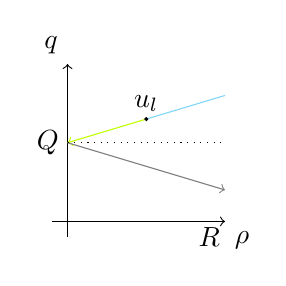
\begin{tikzpicture}
% coordinates
\draw[->] (0,-0.2) -- (0,2) node[anchor= south east] {$q$};
\draw[->] (-0.2,0) -- (2,0) node[anchor= north west] {$\rho$};
% rarefactions

\draw[cyan!50] (1, 1.3) -- (2, 1.6) ;
\draw[<-][lime] (0, 1) -- (1, 1.3) ;
\draw[->][black!50] (0, 1) -- (2, 0.4) ;
\draw[dotted] (0,1) -- (2, 1);
\filldraw[black] (1,1.3) circle (0.5pt) ;
\node at (1, 1.5) {$u_l$};
\node at (1.8, -0.2) {$R$};
\node at (-0.25, 1) {$Q$};
\end{tikzpicture}
\caption{Lax entropy for $q > Q$. \\ Rarefaction (blue) and shock (green).}
\label{Fig:LaxEntropy1CongestedPhase}
\end{minipage}
\quad \quad \quad \quad 
\begin{minipage}{.35\textwidth}
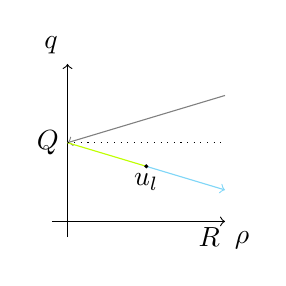
\begin{tikzpicture}
% coordinates
\draw[->] (0,-0.2) -- (0,2) node[anchor= south east] {$q$};
\draw[->] (-0.2,0) -- (2,0) node[anchor= north west] {$\rho$};
% rarefactions
\draw[<-][black!50] (0, 1) -- (2, 1.6) ;
\draw[->][cyan!50] (1,0.7) -- (2, 0.4) ;
\draw[-][lime] (0, 1) -- (1,0.7) ;
\draw[dotted] (0,1) -- (2, 1);
\filldraw[black] (1,0.7) circle (0.5pt) ;
\node at (1, 0.5) {$u_l$};
\node at (1.8, -0.2) {$R$};
\node at (-0.25, 1) {$Q$};
\end{tikzpicture}
\caption{Lax entropy for $q < Q$ \\ Rarefaction (blue) and shock (green).}
\label{Fig:LaxEntropy2CongestedPhase}
\end{minipage}
\end{figure}

Investigating what happens above the critical line $ q = Q$ we see we have a shock when moving towards $u_l$. 
Below the line we also have shock when moving towards $u_l$ . Colombo summarised this result nicely in \cite{Colombo2002}. \begin{align}
   & \begin{cases}
    \nabla \lambda_1 \cdot r_1 < 0 \\
    q > Q
    \end{cases} \iff \begin{cases}
    \text{Braking} \leftrightarrow \text{Shock} \\
    \text{Accelerating} \leftrightarrow \text{Rarefaction} 
    \end{cases} \\
   &\begin{cases}
    \nabla \lambda_1 \cdot r_1 > 0 \\
    q < Q
    \end{cases} \iff \begin{cases}
    \text{Braking} \leftrightarrow \text{Rarefaction} \\
    \text{Accelerating} \leftrightarrow \text{Shock} 
    \end{cases}
    \label{LaxentropySummarised}
\end{align} From the result above \ref{LaxentropySummarised}, we have now acquired criteria $5.$ for realistic traffic flow. 

From an experimental point of view we can now estimate the parameters $Q_1, Q_2$, and $Q$. 

%We can also reformulate the solution curves in the $(\rho, \rho v)$-plane, for both the congested phase and free phase. 

\paragraph{The Riemann Problem.}
We have now all the necessary details to solve the Riemann Problem in the congested phase. Assume $(u_l, u_r) \in \Omega_c, u = (\rho, q)$ and the following initial data: 

\begin{align*}
    (\rho, q) (0,x) = \begin{cases}
    (\rho_l, q_l), \quad  x < 0 \\
    (\rho_r, q_r), \quad  x \geq 0
    \end{cases}
    %\label{Eq:Riemann_init_phaseTr}
\end{align*}

We have two wave curve families. The slow(first) family, 

\begin{align}
     W_1(u_l) = \begin{cases}
     \frac{\rho( q_l - Q)}{\rho_l} + Q, \quad \textit{Rarefaction}\\
     \frac{\rho( q_l - Q)}{\rho_l} + Q,  \quad \textit{Shock} \\
     \quad Q, \quad \forall u(q_l=Q, \rho) \quad \textit{Contact Discontinuity}
     \end{cases}
\end{align}

And the fast(second) family 

\begin{align}
     W_2(u_l) = \begin{cases}
     \frac{\rho( R - \rho_l)}{\rho_l( R - \rho)}, \forall u > 0  \quad \textit{Contact discontinuity}
     \end{cases}
\end{align}

We always have to move in the direction of increasing $\lambda$, this makes us travel from left state along the slow wave to a middle state, and follow by a fast wave to the right state. If $u_l, u_r \in W_1(u_l)$ then the solution is only a slow first wave $W_1(u_l)$ to $u_r$, for shock, rarefaction and contact discontinuity if $u_l(\rho, q_l = Q)$. This also holds for $u_l, u_r \in W_2(u_l)$, then the solution is only a fast second family wave from $u_l$ to $u_r$. 

We have proved Proposition $2.1$ in \cite{Colombo2002}. We state the result below.

\begin{proposition}
Fix positive $Q, R, V$, and let $\rho > 0$ . For all $(\rho_l, q_l)$ and $(\rho_r, q_r)$ in $\Omega_c$, the Riemann problem \begin{align}
    &\begin{cases}
    \rho_t + (\rho v )_x = 0 , \\
    q_t + ((q-Q)v)_x = 0 
    \end{cases}  \quad \quad \quad \quad  (\rho, q) (0,x) = \begin{cases}
    (\rho_l, q_l), \quad  x < 0 \\
    (\rho_r, q_r), \quad  x \geq 0
    \end{cases} \\
    & v = v_c(\rho,q) = \big(1 - \frac{\rho}{R}\big)\frac{q}{\rho}
    \label{Eq:phase-tranision}
\end{align}admits a unique self-similar solution consisting of a slow wave $W_1(u_l)$ between  $(\rho_l, q_l)$ and  $(\rho_m, q_m)$, followed by a fast contact discontinuity  $W_2(u_m)$ between  $(\rho_m, q_m)$ and  $(\rho_r, q_r)$. The slow wave is present whenever $v_c(\rho_l, q_l) \neq v_c(\rho_r, q_r)$ and is either a shock, rarefaction or a contact discontinuity. The latter case if and only if $q_l = Q$. In all cases, the solution attains values in $\Omega_c$.

\end{proposition}
Note we require $\rho > 0$ for well-posedness, as the contact discontinuity is undefined for $\rho = 0$. However, this will not be a problem when investigating the full model, as a phase-transition into a free phase will occur when we approach low density. 

\begin{figure} \centering
\begin{minipage}{.3\textwidth}
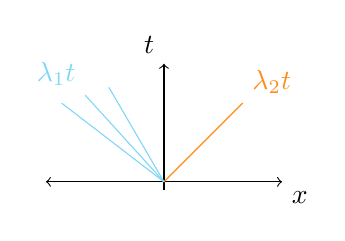
\begin{tikzpicture}
% coord.
\draw[<->] (-1.5,0) -- (1.5,0) node[anchor= north west] {$x$};
\draw[->] (0,-0.1) -- (0,1.5) node[anchor=south east] {$t$};
% contact disc
\draw[color=orange!90!white] (0,0) -- (1,1) node[anchor= south west] {$\lambda_2 t$};
% rarefaction
\draw[color=cyan!50!white] (0,0) -- (-1.3,1);
\draw[color=cyan!50!white] (0,0) -- (-1,1.1) node[anchor= south east] {$\lambda_1 t$};
\draw[color=cyan!50!white] (0,0) -- (-0.7,1.2);
\end{tikzpicture}
\caption{Slow rarefaction (blue) followed by a contact discontinuity (orange)}
\label{Fig:SolRPRarefactionDiscCongestedPhase}
\end{minipage}
\begin{minipage}{.3\textwidth}
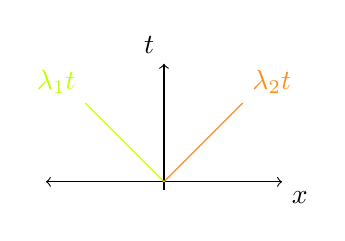
\begin{tikzpicture}
\draw[<->] (-1.5,0) -- (1.5,0) node[anchor= north west] {$x$};
\draw[->] (0,-0.1) -- (0,1.5) node[anchor=south east] {$t$};
\draw[color=orange!90!white] (0,0) -- (1,1) node[anchor= south west] {$\lambda_2 t$};
\draw[color=lime] (0,0) -- (-1,1) node[anchor= south east] {$\lambda_1 t$};
\end{tikzpicture}
\caption{Slow shock (green) followed by a contact discontinuity (orange)}
\label{Fig: SolRPShockDiskCongestedPhase}
\end{minipage}
\begin{minipage}{.3\textwidth}
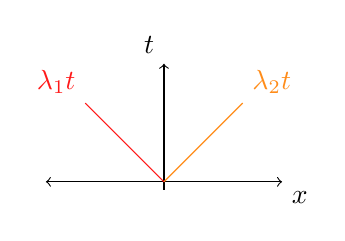
\begin{tikzpicture}
\draw[<->] (-1.5,0) -- (1.5,0) node[anchor= north west] {$x$};
\draw[->] (0,-0.1) -- (0,1.5) node[anchor=south east] {$t$};
\draw[color=orange!90!white] (0,0) -- (1,1) node[anchor= south west] {$\lambda_2 t$};
\draw[color=red!90!white] (0,0) -- (-1,1) node[anchor= south east] {$\lambda_1 t$};
\end{tikzpicture}
\caption{Contact discontinuity followed by a contact discontinuity, $q_l = Q$}
\label{Fig: SolRPDiscCongestedPhase}
\end{minipage}
\end{figure}

We will now demonstrate possible solutions.

% ---- TIKZ FIGURE -----
\vspace{6pt}
\begin{minipage}{.2\textwidth}
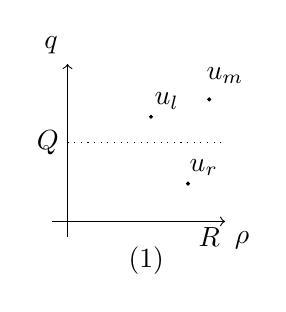
\begin{tikzpicture}
% coordinates
\draw[->] (0,-0.2) -- (0,2) node[anchor= south east] {$q$};
\draw[->] (-0.2,0) -- (2,0) node[anchor= north west] {$\rho$};
% rarefactions
%\draw[cyan!50] (1, 1.3) -- (2, 1.6) ;
%\draw[<-][lime] (0, 1) -- (1, 1.3) ;
%\draw[->][cyan!50] (0, 1) -- (2, 0.4) ;


\draw[cyan!50, domain=0:2]  plot[id=x] function{0.31*x +1};
\draw[cyan!50, domain=0:2]  plot[id=x] function{-0.34*x +1};
\draw[dotted] (0,1) -- (2, 1);
% contact disk
\draw[orange!50, domain=0:1.28]  plot[id=x] function{(x/1.16)*(2-1.16)/(2-x)*1.63};
\draw[orange!50, domain=0:1.86]  plot[id=x] function{(x/1.38)*(2-1.38)/(2-x)*0.33};
% initial conditions
\node at (1.06+0.2, 1.33+0.2) {$u_l$};
\node at (1.53+0.2, 0.48+0.2) {$u_r$};
\node at (1.8+0.2, 1.55+0.3) {$u_m$};
\filldraw[black] (1.06, 1.33) circle (0.5pt);  % u_1
\filldraw[black] (1.53, 0.48) circle (0.5pt);   % u_2
\filldraw[black] (1.8, 1.55) circle (0.5pt);   % u_m
%labels
\node at (1.8, -0.2) {$R$};
\node at (-0.25, 1) {$Q$};
\node at (1, -0.5) {$(1)$};
\end{tikzpicture}
\end{minipage}
\begin{minipage}{.2\textwidth}
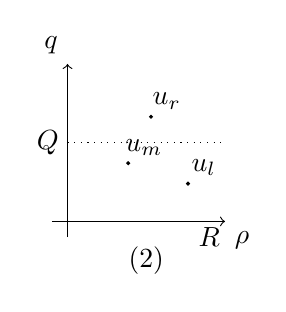
\begin{tikzpicture}
% coordinates
\draw[->] (0,-0.2) -- (0,2) node[anchor= south east] {$q$};
\draw[->] (-0.2,0) -- (2,0) node[anchor= north west] {$\rho$};
% rarefactions
%\draw[cyan!50] (1, 1.3) -- (2, 1.6) ;
%\draw[<-][lime] (0, 1) -- (1, 1.3) ;
%\draw[->][cyan!50] (0, 1) -- (2, 0.4) ;
\draw[cyan!50, domain=0:2]  plot[id=x] function{0.31*x +1};
\draw[lime, domain=0:2]  plot[id=x] function{-0.34*x +1};
\draw[dotted] (0,1) -- (2, 1);
% contact disk
\draw[orange!50, domain=0:1.28]  plot[id=x] function{(x/1.16)*(2-1.16)/(2-x)*1.63};
\draw[orange!50, domain=0:1.86]  plot[id=x] function{(x/1.38)*(2-1.38)/(2-x)*0.33};
% initial conditions
\node at (1.06+0.2, 1.33+0.2) {$u_r$};
\node at (1.53+0.2, 0.48+0.2) {$u_l$};
\node at (0.77+0.2, 0.74+0.2) {$u_m$};
\filldraw[black] (0.77, 0.74) circle (0.5pt);   % u_m
\filldraw[black] (1.06, 1.33) circle (0.5pt);  % u_1
\filldraw[black] (1.53, 0.48) circle (0.5pt);   % u_2
%labels
\node at (1.8, -0.2) {$R$};
\node at (-0.25, 1) {$Q$};
\node at (1, -0.5) {$(2)$};
\end{tikzpicture}
\end{minipage}
\quad
\begin{minipage}{.2\textwidth}
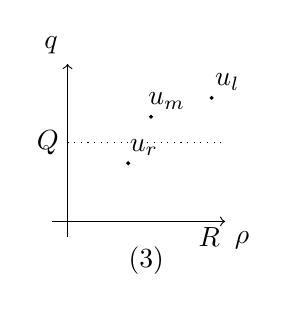
\begin{tikzpicture}
% coordinates
\draw[->] (0,-0.2) -- (0,2) node[anchor= south east] {$q$};
\draw[->] (-0.2,0) -- (2,0) node[anchor= north west] {$\rho$};
% rarefactions
%\draw[cyan!50] (1, 1.3) -- (2, 1.6) ;
%\draw[<-][lime] (0, 1) -- (1, 1.3) ;
%\draw[->][cyan!50] (0, 1) -- (2, 0.4) ;
\draw[lime, domain=0:2]  plot[id=x] function{0.31*x +1};
\draw[cyan!50, domain=0:2]  plot[id=x] function{-0.34*x +1};
\draw[dotted] (0,1) -- (2, 1);
% contact disk
\draw[orange!50, domain=0:1.28]  plot[id=x] function{(x/1.16)*(2-1.16)/(2-x)*1.63};
\draw[orange!50, domain=0:1.86]  plot[id=x] function{(x/1.38)*(2-1.38)/(2-x)*0.33};
% initial conditions
\node at (1.83+0.2, 1.57+0.2) {$u_l$};
\node at (0.77+0.2, 0.74+0.2) {$u_r$};
\node at (1.06+0.2, 1.33+0.2) {$u_m$};
\filldraw[black] (1.83, 1.57) circle (0.5pt);  % u_1
\filldraw[black] (0.77, 0.74) circle (0.5pt);   % u_2
\filldraw[black] (1.06, 1.33) circle (0.5pt);  % u_m
%labels
\node at (1.8, -0.2) {$R$};
\node at (-0.25, 1) {$Q$};
\node at (1, -0.5) {$(3)$};
\end{tikzpicture}
\end{minipage}
\begin{minipage}{.2\textwidth}
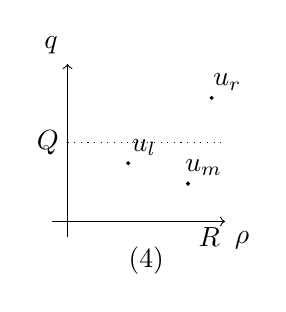
\begin{tikzpicture}
% coordinates
\draw[->] (0,-0.2) -- (0,2) node[anchor= south east] {$q$};
\draw[->] (-0.2,0) -- (2,0) node[anchor= north west] {$\rho$};
% rarefactions
%\draw[cyan!50] (1, 1.3) -- (2, 1.6) ;
%\draw[<-][lime] (0, 1) -- (1, 1.3) ;
%\draw[->][cyan!50] (0, 1) -- (2, 0.4) ;
\draw[cyan!50, domain=0:2]  plot[id=x] function{0.31*x +1};
\draw[cyan!50, domain=0:2]  plot[id=x] function{-0.34*x +1};
\draw[dotted] (0,1) -- (2, 1);
% contact disk
\draw[orange!50, domain=0:1.28]  plot[id=x] function{(x/1.16)*(2-1.16)/(2-x)*1.63};
\draw[orange!50, domain=0:1.86]  plot[id=x] function{(x/1.38)*(2-1.38)/(2-x)*0.33};
% initial conditions
\node at (1.83+0.2, 1.57+0.2) {$u_r$};
\node at (0.77+0.2, 0.74+0.2) {$u_l$};
\node at (1.53+0.2, 0.48+0.2) {$u_m$};
\filldraw[black] (1.83, 1.57) circle (0.5pt);  % u_1
\filldraw[black] (0.77, 0.74) circle (0.5pt);   % u_2
\filldraw[black] (1.53, 0.48) circle (0.5pt);  % u_m
%labels
\node at (1.8, -0.2) {$R$};
\node at (-0.25, 1) {$Q$};
\node at (1, -0.5) {$(4)$};
\end{tikzpicture}
\end{minipage}
\vspace{6pt}

\begin{align*}
    u_1(x,t) = \begin{cases}
    u_l, x < \lambda_1(u_l)t\\
    W_1, \lambda_1(u_l)t < x < \lambda_1(u_r)t, \quad \textit{Raref.}\\ 
    u_m, \lambda_1(u_r)t < x < \lambda_2(u_l)t \\
    W_2, \lambda_2(u_l)t < x < \lambda_2(u_r)t \quad \textit{Contact D.} \\
    u_r, x < \lambda_2(u_r)t \\
    \end{cases}
    u_2(x,t) = \begin{cases}
    u_l, x < \lambda_1(u_l)t\\
    W_1, \lambda_1(u_l)t < x < \lambda_1(u_r)t, \quad \textit{Shock}\\ 
    u_m, \lambda_1(u_r)t < x < \lambda_2(u_l)t \\
    W_2, \lambda_2(u_l)t < x < \lambda_2(u_r)t \quad \textit{Contact D.} \\
    u_r, x < \lambda_2(u_r)t \\
    \end{cases}
\end{align*}

\begin{align*}
    u_3(x,t) = \begin{cases}
    u_l, x < \lambda_1(u_l)t\\
    W_1, \lambda_1(u_l)t < x < \lambda_1(u_r)t, \quad \textit{Shock}\\ 
    u_m, \lambda_1(u_r)t < x < \lambda_2(u_l)t \\
    W_2, \lambda_2(u_l)t < x < \lambda_2(u_r)t \quad \textit{Contact D.} \\
    u_r, x < \lambda_2(u_r)t \\
    \end{cases}
    u_4(x,t) = \begin{cases}
    u_l, x < \lambda_1(u_l)t\\
    W_1, \lambda_1(u_l)t < x < \lambda_1(u_r)t, \quad \textit{Raref.}\\ 
    u_m, \lambda_1(u_r)t < x < \lambda_2(u_l)t \\
    W_2, \lambda_2(u_l)t < x < \lambda_2(u_r)t \quad \textit{Contact D.} \\
    u_r, x < \lambda_2(u_r)t \\
    \end{cases}
\end{align*}

\begin{align*}
    u_5(x,t) = \begin{cases}
    u_l, x < \lambda_1(u_l)t\\
    W_1, \lambda_1(u_l)t < x < \lambda_1(u_r)t, \quad \textit{Contact D.}\\ 
    u_m, \lambda_1(u_r)t < x < \lambda_2(u_l)t \\
    W_2, \lambda_2(u_l)t < x < \lambda_2(u_r)t \quad \textit{Contact D.} \\
    u_r, x < \lambda_2(u_r)t \\
    \end{cases}
\end{align*}


\begin{wrapfigure}[11]{R}{0.2\textwidth}
    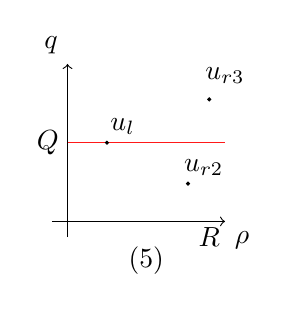
\begin{tikzpicture}
    % coordinates
    \draw[->] (0,-0.2) -- (0,2) node[anchor= south east] {$q$};
    \draw[->] (-0.2,0) -- (2,0) node[anchor= north west] {$\rho$};
    % disc
    \draw[red!90!white] (0,1) -- (2, 1);
    % contact disk
    %\draw[orange!50, domain=0:1.28]  plot[id=x] function{(x/1.16)*(2-1.16)/(2-x)*1.63};
    \draw[orange!50, domain=0:1.86]  plot[id=x] function{(x/1.38)*(2-1.38)/(2-x)*0.33};
    % initial conditions
    \node at (0.5+ 0.2, 1+0.2) {$u_l$};
    %\node at (1.06+0.2, 1.33+0.2) {$u_1$};
    \node at (1.53+0.2, 0.48+0.2) {$u_{r2}$};
    \node at (1.8+0.2, 1.55+0.3) {$u_{r3}$};
    %\node at (0.77+0.2, 0.74+0.2) {$u_4$};
    \filldraw[black] (0.5, 1) circle (0.5pt);   % u_m
    %\filldraw[black] (0.77, 0.74) circle (0.5pt);   % u_m
    %\filldraw[black] (1.06, 1.33) circle (0.5pt);  % u_1
    \filldraw[black] (1.53, 0.48) circle (0.5pt);   % u_2
    \filldraw[black] (1.8, 1.55) circle (0.5pt);   % u_m
    %labels
    \node at (1.8, -0.2) {$R$};
    \node at (-0.25, 1) {$Q$};
    \node at (1, -0.5) {$(5)$};
    \end{tikzpicture}
    \caption{Discontinuity solutions}
    \label{Fig:u_5}
\end{wrapfigure}

Note that only if $u_l$ with $(\rho, q_l = Q)$ starts the first wave family as a contact discontinuity. If $u_r$ is on $q = Q$ then either it is the end of the first family contact discontinuity or the end of the second wave contact discontinuity which happens to be on $u_r(\rho, q_r = Q)$.



\subsection{The Riemann Problem for the full model}
We will now combine the two sets of equations and solve the system including phase-transitions. If both $u_l, u_r \in \Omega_f$ then the solution is given in section \ref{RPFreePh}, and if $u_l, u_r \in \Omega_c$ then the solution is given in section \ref{RPCongPh}. Thus, in this section we will only deal with the cases $u_l \in \Omega_f, u_r \in \Omega_c$ and $u_l \in \Omega_c, u_r \in \Omega_f$.

%Entropy for phase transitions
Colombo gives an entopy condition necessary for phase transitions in section 3 in \cite{Colombo2003}, and the requirement is as follows: If $u_l \in \Omega_f$ and $u_r \in \Omega_c$ then an \textit{admissible solution} to \ref{Eq:phase-transition} is a self-similar function $u:[0, \infty) \times \mathbb{R} \mapsto \Omega_f \cup \Omega_c$ such that there exists a $\Lambda \in \mathbb{R}$ with 
\begin{enumerate}
    \item $u:(t, (-\infty,\Lambda t)) \subseteq \Omega_f $ and $u:(t, (\Lambda t, \infty)) \subseteq \Omega_c $ 
    \item the functions $u_l$ and $u_r$ respectively defined by \begin{align*}
        & u_l(t,x) = \begin{cases}
        u(t,x),  \quad x < \Lambda t\\
        u(t,\Lambda t-),\quad x > \Lambda t
        \end{cases}
        & u_r(t,x) = \begin{cases}
        u(t,\Lambda t+), \quad x < \Lambda t\\
        u(t,x), \quad x > \Lambda t
        \end{cases}
    \end{align*} are restrictions of Lax solutions to the scalar and systems case respectively. 
    \item the Rankine-Hugoniot conditions 
    \begin{align}
        \Lambda (\rho (t,\Lambda t+) - \rho (t,\Lambda t-)) = \rho (t,\Lambda t+) v_c(t,\Lambda t+) - \rho (t,\Lambda t-) v_f(t,\Lambda t-)
        \label{RH_PhT}
    \end{align} are satisfied for all $t \geq 0$
    
\end{enumerate}

%\todo{If V_c = V_f}

\paragraph{Generalised Riemann coordinates.}
We generalise to Riemann coordinates. 
\begin{definition}[Riemann invariants]
A smooth function $\omega : \mathbb{R}^n \mapsto \mathbb{R}$ is called a \textit{k-Riemann invariant} if 
\begin{align*}
    \nabla \omega(u) \cdot r_k (u) = 0
\end{align*}
where $r_k$ is the k'th right eigenvector of the strictly hyperbolic Jacobian $df$.
\end{definition}
From the definition of Riemann invariants one can show that the rarefaction curves are constant on all Riemann invariants, and thus we can use this as an alternative definition of rarefaction. 
Let $\hat u = (\hat R, \hat Q)$ be the point in $\Omega_f$ defined by $\hat Q = \hat R V$, see Figure \ref{Domain congested ph}. The point $\hat u$ lies on the continuation of the lower border of $\Omega_c$.  
For $\Omega_f$ we have \todo{$\Omega_f$ riemann coord.}\\
For $\Omega_c$ we have the right eigenvectors
\begin{align*}
    &\lambda_1 = \big ( \frac{2}{R} - \frac{1}{\rho} )\big (Q- q) - \frac{Q}{R}, \quad \quad \lambda_2 = \big(1 - \frac{\rho}{q}\big)\frac{q}{\rho} = v_c \\
    & r_1 = \begin{pmatrix} \rho \\ q - Q \end{pmatrix} \quad \quad \quad  \quad \quad \quad \quad \quad  r_2 = \begin{pmatrix} R - \rho \\ \frac{Rq}{\rho} \end{pmatrix} \\
    & \nabla \lambda_1 \cdot r_1 = 2\frac{Q-q}{R} \quad \quad \quad \quad \quad  \quad \nabla \lambda_2 \cdot r_2 = 0
\end{align*}
Note we have already found $\nabla \lambda_2 \cdot r_2 = 0$, we choose this as $\omega_1 = \lambda_2 = v_c$. For $\nabla \omega_2 \cdot r_1 = \big ( \frac{\partial \omega_2}{\partial \rho}, \frac{\partial \omega_2}{\partial q} \big ) \cdot \begin{pmatrix} \rho \\ q - Q \end{pmatrix} = 0 $ we see that by choosing  $\frac{\partial \omega_2}{\partial \rho} = - \frac{ q-Q }{\rho}$ and $ \frac{\partial \omega_2}{\partial q} =  \frac{1}{\rho} $ the expressions cancel. Now we have    $\omega_2 = \frac{q-Q}{\rho}$, which is a desirable result as it the slope of the first family wave. 

Now we have the Riemann coordinates
\begin{align*}
    \omega_1 = \begin{cases}
    v_c(\rho, q), (\rho, q) \in \Omega_c \\
    V_f, (\rho, q) \in \Omega_f
    \end{cases}
    \omega_2 = \begin{cases}
    \frac{q-Q}{\rho}, (\rho, q) \in \Omega_c \\
    \frac{q-Q}{\rho}, (\rho, q) \in \Omega_f, \rho \geq \hat R \\
    v_f(\rho) - v_f(\hat R) + \frac{\hat Q - Q}{\hat R }, (\rho, q) \in \Omega_f, \rho \leq \hat R \\
    \end{cases}
\end{align*}

We continue by finding the direction of the rarefaction and shock in the new coordinate system. 

\begin{figure} \centering 
\begin{minipage}{.35\textwidth}
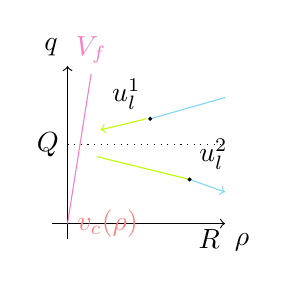
\begin{tikzpicture}
% coordinates
\draw[->] (0,-0.2) -- (0,2) node[anchor= south east] {$q$};
\draw[->] (-0.2,0) -- (2,0) node[anchor= north west] {$\rho$};
% rarefactions
\draw[cyan!50] (1.05, 1.33) -- (2, 1.6) ;
\draw[<-][lime] (0.42, 1.19) -- (1, 1.33) ;

\draw[->][cyan!50] (1.55,0.56)  -- (2, 0.4) ;
\draw[-][lime] (0.37, 0.85) -- (1.55,0.56)  ;

% v_c
\draw[red!50, domain=0:0.69]  plot[id=x] function{x*(3*x+1)}  node[right] {$v_c(\rho)$};
% V_f
\draw[magenta!50] (0,0) -- (0.3, 1.9);
\node[magenta!50] at (0.3, 2.2) {$V_f$};

\draw[dotted] (0,1) -- (2, 1);
\filldraw[black] (1.05,1.33) circle (0.5pt) node[anchor = south east]{$u_l^1$} ;
\filldraw[black] (1.55,0.56) circle (0.5pt) node[anchor = south west]{$u_l^2$} ;
% contacts
\draw[ orange!50, domain=0:1.86]  plot[id=x] function{(x/1.38)*(2-1.38)/(2-x)*0.33};
\draw[ orange!50, domain=0:1.28]  plot[id=x] function{(x/1.16)*(2-1.16)/(2-x)*1.63};
%
%\node at (1, 1.55) {$u_l$};
\node at (1.8, -0.2) {$R$};
\node at (-0.25, 1) {$Q$};
\end{tikzpicture}
\caption{Wave solutions from two starting points $u_l^1$ and $u_l^2$. }
\label{Fig:FullSol_ic_rhoq}
\end{minipage}
\quad \quad \quad \quad 
\begin{minipage}{.35\textwidth}
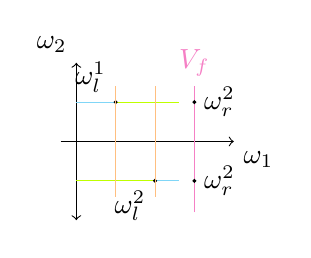
\begin{tikzpicture}
% coordinates
\draw[<->] (0,0) -- (0,2) node[anchor= south east] {$\omega_2$};
\draw[->] (-0.2,1) -- (2,1) node[anchor= north west] {$\omega_1$};
% rarefactions
% rarefactions
\draw[cyan!50] (0, 1.5) -- (0.5, 1.5) ;
\draw[lime] (0.5, 1.5) -- (1.3, 1.5)  ;
\filldraw[black] (0.5, 1.5) circle (0.5pt) node[anchor = south east]{$\omega_l^1$} ;

\draw[lime] (0, 0.5) -- (1, 0.5) ;
\draw[cyan!50] (1, 0.5) -- (1.3, 0.5) ;
\filldraw[black] (1, 0.5)  circle (0.5pt) node[anchor = north east]{$\omega_l^2$} ;

% contacts
\draw[orange!50] (0.5, 1.7) -- (0.5, 0.3) ;
\draw[orange!50] (1, 1.7) -- (1, 0.3) ;

% free ph line
\draw[magenta!50] (1.5, 0.1) -- (1.5, 1.7); 
\node[magenta!50] at (1.5, 2) {$V_f$};
\filldraw[black] (1.5, 1.5)  circle (0.5pt) node[anchor =  west]{$\omega_r^2$} ;
\filldraw[black] (1.5, 0.5)  circle (0.5pt) node[anchor = west]{$\omega_r^2$} ;

\end{tikzpicture}
\caption{Wave solutions from two starting points $\omega_l^1$ and $\omega_l^2$.}
\label{Fig:FullSol_ic_ww}
\end{minipage}
\end{figure}

From Figure \ref{Fig:FullSol_ic_rhoq}, observe that
\begin{align*}
    q > Q \begin{cases}
    q \searrow rarefaction\\
    q \nearrow shock
    \end{cases}
    q > Q \begin{cases}
    q \searrow shock \\
    q \nearrow rarefaction
    \end{cases}
\end{align*}

Using the relation between the coordinates $\rho, q$ and $\omega_1, \omega_2$ 
\begin{itemize}
    \item $\omega_2 > 0$ 
    $\rho$ const. $q \searrow \leftrightarrow \omega_1, \omega_2 \searrow$ rarefaction
    \item $\omega_2 < 0$ 
    $\rho$ const. $q \searrow \leftrightarrow \omega_1, \omega_2 \searrow$ shock
\end{itemize}

Which means we have the relation between shock and rarefaction in $\omega$-coordinates, the result can be seen in Figure \ref{Fig:FullSol_ic_ww}
\begin{align*}
    \omega_2 > 0 \begin{cases}
    \omega_2 \searrow rarefaction\\
    \omega_2 \nearrow shock
    \end{cases}
    \omega_2 < 0\begin{cases}
    \omega_2 \searrow shock \\
    \omega_2 \nearrow rarefaction
    \end{cases}
\end{align*}

\paragraph{Generalised Lax curves.}
\todo{}
What happens on the boundary between two phases, how can I show shock and raref. or disc? 

Let $\omega_l^1, \omega_l^2 \in \Omega_c$, and $\omega_r^1, \omega_r^2 \in \Omega_f$. The entropy-admissible solution from
\begin{itemize}
    \item $\omega_l^1$ to $\omega_r^1$ is given by a rarefaction wave followed by a phase transition
    \item $\omega_l^2$ to $\omega_r^2$ is given by a shock-like phase transition
    \item If $\omega_l = 0$, and $\omega_r = 0$ then the solution is a phase transition acting as a contact discontinuity. 
\end{itemize}

And recall that the speed of the phase boundary is assigned by the Rankine-Hugoniot condition for phase transitions \ref{RH_PhT}.

\begin{wrapfigure}[11]{R}{0.2\textwidth}
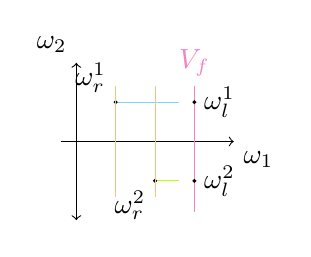
\begin{tikzpicture}
% coordinates
\draw[<->] (0,0) -- (0,2) node[anchor= south east] {$\omega_2$};
\draw[->] (-0.2,1) -- (2,1) node[anchor= north west] {$\omega_1$};
% rarefactions
%\draw[cyan!50] (0, 1.5) -- (0.5, 1.5) ;
\draw[cyan!50] (0.5, 1.5) -- (1.3, 1.5)  ;
\filldraw[black] (0.5, 1.5) circle (0.5pt) node[anchor = south east]{$\omega_r^1$} ;

%\draw[lime] (0, 0.5) -- (1, 0.5) ;
\draw[lime] (1, 0.5) -- (1.3, 0.5) ;
\filldraw[black] (1, 0.5)  circle (0.5pt) node[anchor = north east]{$\omega_r^2$} ;

% contacts
\draw[orange!50] (0.5, 1.7) -- (0.5, 0.3) ;
\draw[orange!50] (1, 1.7) -- (1, 0.3) ;

% free ph line
\draw[magenta!50] (1.5, 0.1) -- (1.5, 1.7); 
\node[magenta!50] at (1.5, 2) {$V_f$};
\filldraw[black] (1.5, 1.5)  circle (0.5pt) node[anchor =  west]{$\omega_l^1$} ;
\filldraw[black] (1.5, 0.5)  circle (0.5pt) node[anchor = west]{$\omega_l^2$} ;

\end{tikzpicture}
\caption{Wave solutions from two starting points $\omega_l^1$ and $\omega_l^2$.}
\label{Fig:FullSol_ic_ww2}
\end{wrapfigure}

Let $\omega_l^1, \omega_l^2 \in \Omega_f$, and $\omega_r^1, \omega_r^2 \in \Omega_c$. The entropy-admissible solution from
\begin{itemize}
    \item $\omega_l^1$ to $\omega_r^1$  is given by a shock-like phase transition.
    \item $\omega_l^2$ to $\omega_r^2$ is given by a phase transition followed by a rarefaction wave
    \item If $\omega_l = 0$, and $\omega_r = 0$ then the solution is a phase transition acting as a contact discontinuity. 
\end{itemize}


%\begin{wrapfigure}[9]{L}{0.4\textwidth}
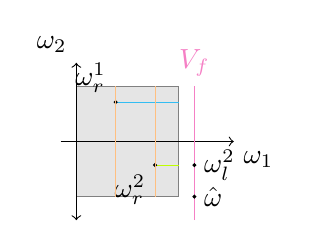
\begin{tikzpicture}
% coordinates
% Omega_c
\filldraw[fill=black!10!white, draw=black!50] plot [tension = 1] coordinates { (0,1.7) (1.3,1.7) (1.3,0.3) (0, 0.3) };
\draw[<->] (0,0) -- (0,2) node[anchor= south east] {$\omega_2$};
\draw[->] (-0.2,1) -- (2,1) node[anchor= north west] {$\omega_1$};
% rarefactions
%\draw[cyan!50] (0, 1.5) -- (0.5, 1.5) ;

\draw[cyan!80] (0.5, 1.5) -- (1.3, 1.5)  ;
\filldraw[black] (0.5, 1.5) circle (0.5pt) node[anchor = south east]{$\omega_r^1$} ;

%\draw[lime] (0, 0.5) -- (1, 0.5) ;
\draw[lime] (1, 0.7) -- (1.3, 0.7) ;
\filldraw[black] (1, 0.7)  circle (0.5pt) node[anchor = north east]{$\omega_r^2$} ;

% contacts
\draw[orange!50] (0.5, 1.7) -- (0.5, 0.3) ;
\draw[orange!50] (1, 1.7) -- (1, 0.3) ;

% free ph line
\draw[magenta!50] (1.5, 0) -- (1.5, 1.7); 
\node[magenta!50] at (1.5, 2) {$V_f$};
\filldraw[black] (1.5, 0.7)  circle (0.5pt) node[anchor = west]{$\omega_l^2$} ;
\filldraw[black] (1.5, 0.3)  circle (0.5pt) node[anchor = west]{$\hat \omega$} ;

\end{tikzpicture}
%\caption{Wave solutions from two starting points $\omega_l^3$ and $\omega_l^3$.}
%\label{Fig:FullSol_ic_ww3}
%\end{wrapfigure}

Noe let $\omega_l^3 \in \Omega_f$, and $ \omega_r^3 \in \Omega_c$. As $\omega_l^3$ is below the point $\hat \omega$, which is the boundary of the domain $\Omega_c$, we define $q_m(\rho) = Q + \rho/R(Q_1 - Q)$.  The entropy-admissible solution from
\begin{itemize}
    \item $\omega_l^1$ to $\omega_r^1$  is given by a shock-like phase transition.
    \item $\omega_l^2$ to $\omega_r^2$ is given by a phase transition followed by a rarefaction wave
    \item If $\omega_l = 0$, and $\omega_r = 0$ then the solution is a phase transition acting as a contact discontinuity. 
\end{itemize}

\newpage

\section{Conclusion}



\newpage

\appendix
\section{Appendix}

\begin{theorem}[Divergence theorem]
Suppose $\Omega \subset \mathbb{R}$ with piecewise $C^1$ boundary $\partial \Omega$. For a vector field $F \in C^1(\bar \Omega; \mathbb{R}^n)$, 
\begin{equation}
    \int_\Omega \nabla \cdot F d^nx = \int_{\partial \Omega} F \cdot \vec{n} ds
\end{equation}
where $\vec{n} $ is the outward unit normal to $\partial \Omega$.
\label{Thm:Divergence}
\end{theorem}
A proof of this theorem (\ref{Thm:Divergence}) can be found in advanced calculus texts. 


\newpage
\printbibliography

\end{document}


